\documentclass{report}

\usepackage[left=3cm,right=3cm,top=1cm,bottom=2cm]{geometry}
\usepackage{polski}
\usepackage[utf8]{inputenc}
\usepackage{graphicx, float, caption, subcaption, pgfplots, adjustbox}

\newenvironment{absolutelynopagebreak}
{\par\nobreak\vfil\penalty0\vfilneg
	\vtop\bgroup}
{\par\xdef\tpd{\the\prevdepth}\egroup
	\prevdepth=\tpd}

\title{%
	System pisania testów na platformie Android \\
	\large Raport inżynierski}

\author{
	Filip Malinowski\\
	\texttt{filip.malinowski@student.pwr.edu.pl}
	\and
	pod przewodnictwem Promotora dr Witolda Paluszyńskiego\\
	\texttt{witold.paluszynski@pwr.edu.pl}
}
\date{}

\begin{document}

%\maketitle

%\tableofcontents

	
	\chapter{Analiza problemu}
	
		\section{Systemy pisania testów w czasie rzeczywistym}
		Na rynku istnieją już aplikacje częściowo odpowiadające tematowi pracy inżynierskiej. Ich funkcjonalność spełnia pewne aspekty pożądanego systemu jakimi są: wybór odpowiedzi do pytań na ekranie telefonu, przesyłanie odpowiedzi do serwera oraz pobieranie informacji z serwera na aplikację. Najlepszym przykładem jest aplikacja nazywająca się Quizowanie\footnote{https://play.google.com/store/apps/details?id=se.feomedia.quizkampen.pl.lite}. Aplikacja ta pozwala na pobieranie i wyświetlenie pytań z serwera, wyświetlenie możliwych odpowiedzi jako przycisków dla użytkownika oraz wysłanie odpowiedzi do serwera i zweryfikowanie ich. Quizowanie jest aplikacją nastawioną na współzawodnictwo pomiędzy użytkownikami, którzy wspólnie odpowiadają na te same pytania zdobywając przy tym punkty. Kod źródłowy tej aplikacji jest zamknięty.
	
		Inne aplikacje, które można wymienić to English Grammar Test\footnote{https://play.google.com/store/apps/details?id=english.grammar.test.app} lub też sameQuizy\footnote{https://play.google.com/store/apps/details?id=pl.filing.samequizy}. English Grammar Test jest aplikacją bardzo rozbudowaną i ukierunkowaną na prostą naukę języka Angielskiego. Schematy odpowiadania na pytania, wybór odpowiedzi oraz poruszanie się po menu aplikacji są zbliżone do tych, jakie występują w aplikacji Quizowanie. W sameQuizy użytkownik, tak jak w poprzednich aplikacjach, w prosty sposób poprzez naciskanie przycisków wybiera odpowiedzi na zadane na ekranie aplikacji pytania. Kod źródłowy obu tych aplikacji jest zamknięty.
		
		Każda z trzech aplikacji wyróżnia się jednak innym podejściem przy tworzeniu interfejsu użytkownika. English Grammar Test ma prosty i czytelny wygląd. Interfejs aplikacji sameQuizy oprócz wyświetlania pytań i propozycji odpowiedzi, urozmaicony jest wieloma obrazami przyciągającymi wzrok. Interfejs aplikacji Quizowanie ma interfejs pośredni pomiędzy tym jaki można zobaczyć w English Grammar Test i sameQuizy.
		
		Interfejs odpowiada zastosowaniu aplikacji. Aplikacje ukierunkowane na rozrywkę mają kolorowy, zwracający uwagę wygląd. Aplikacje ukierunkowane na naukę mają interfejs prosty i czytelny, a te przeznaczone do gier i rywalizacji mają interfejs bardziej urozmaicony, ale w stopniu takim, który nie pogarsza czytelności treści wyświetlanych na ekranie.
		
		\begin{figure}[ht]
			\centering
			\begin{subfigure}{.3\textwidth}
				\centering
				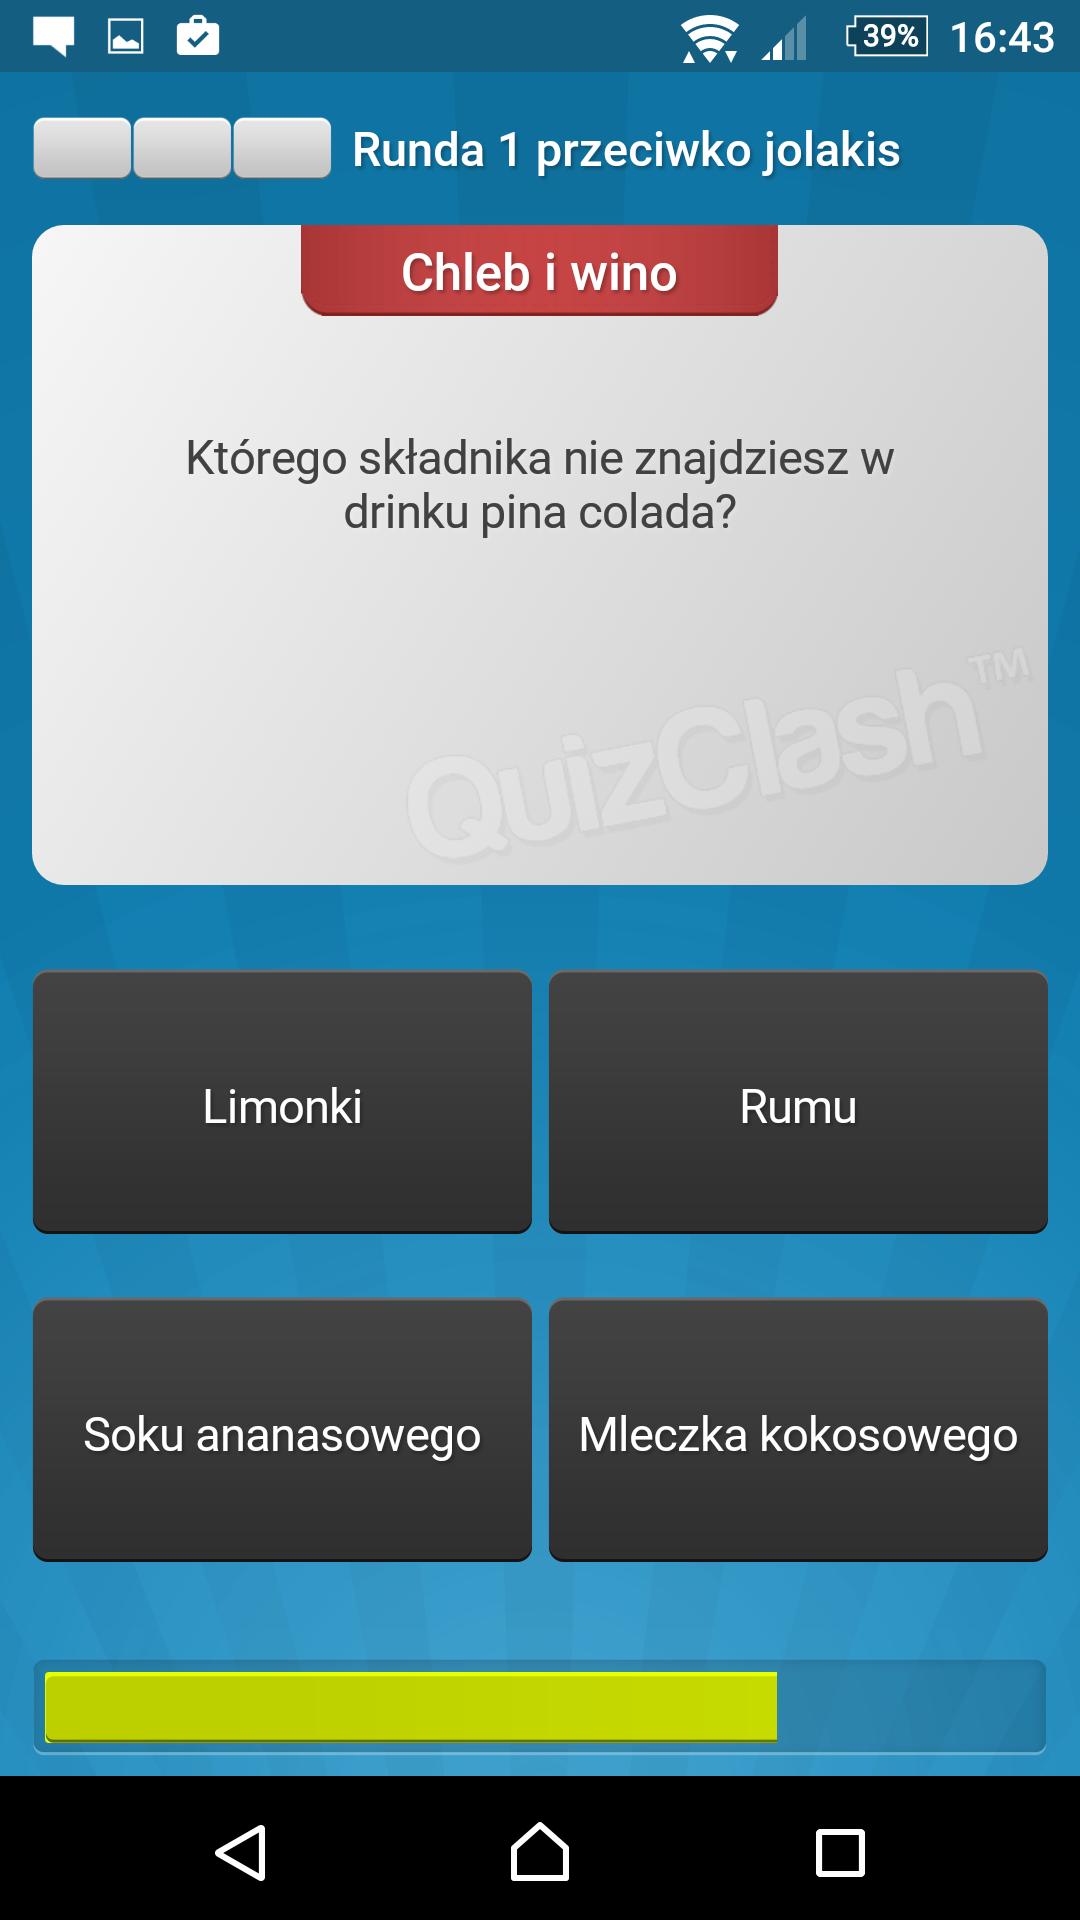
\includegraphics[width=.7\linewidth]{Quizowanie.png}
				\caption{Quizowanie}
				\label{fig:quizowanie}
			\end{subfigure}
			\begin{subfigure}{.3\textwidth}
				\centering
				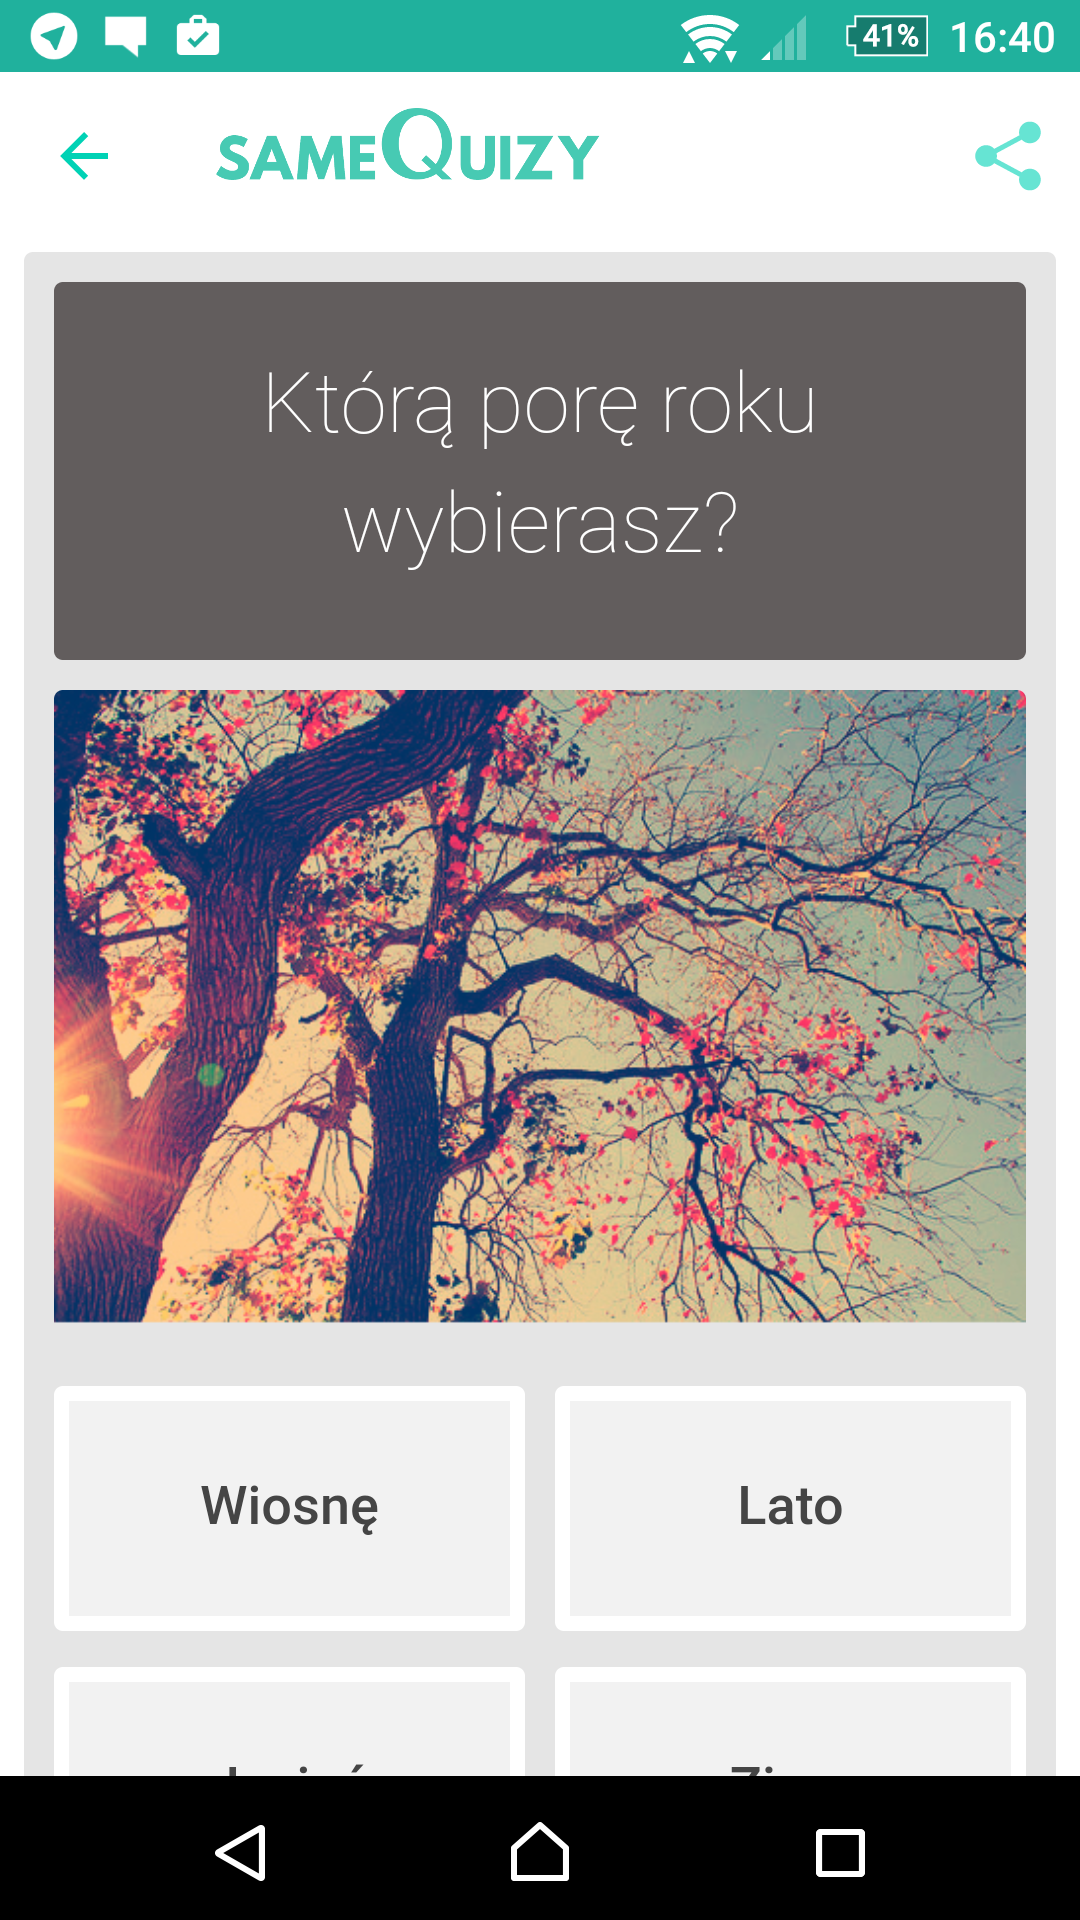
\includegraphics[width=.7\linewidth]{sameQuizy.png}
				\caption{sameQuizy}
				\label{fig:same_quizy}
			\end{subfigure}
			\begin{subfigure}{.3\textwidth}
				\centering
				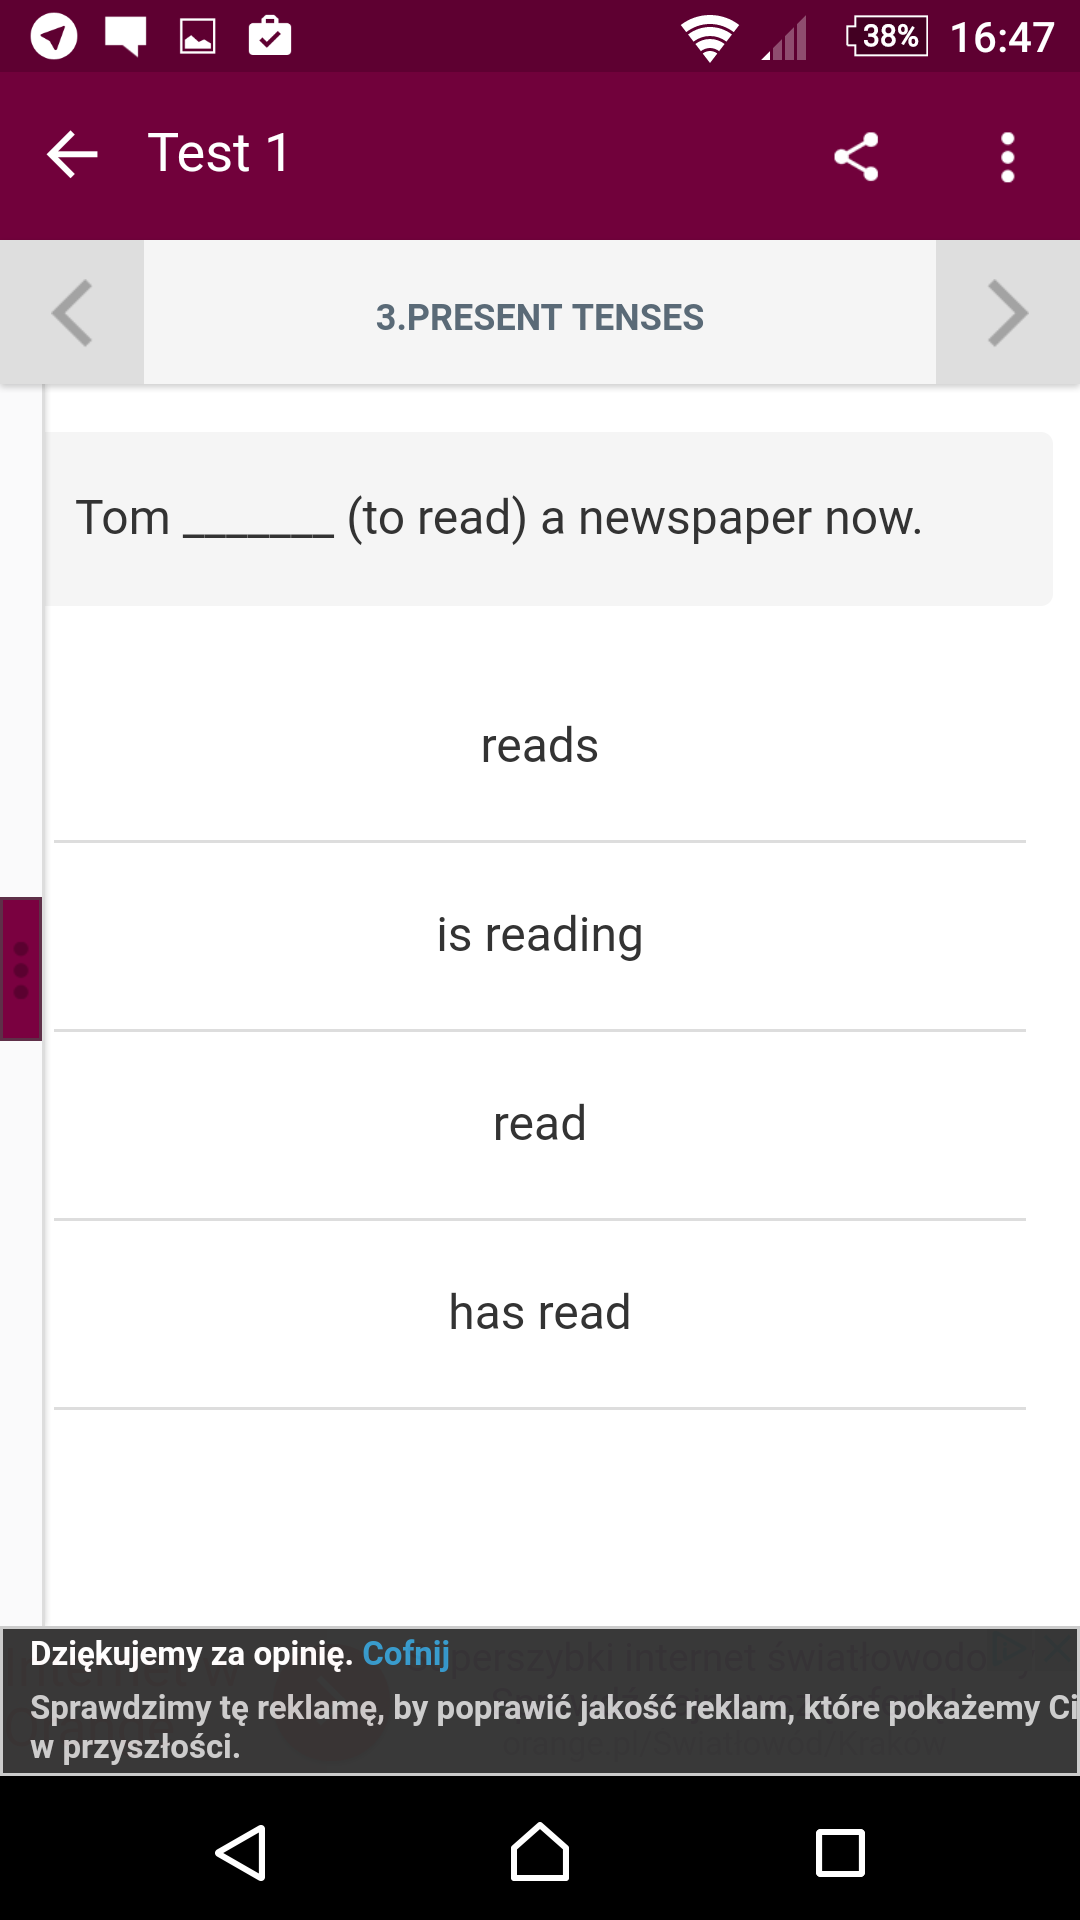
\includegraphics[width=.7\linewidth]{English_Grammar_Test.png}
				\caption{English Grammar Test}
				\label{fig:english_grammar_test}
			\end{subfigure}
			\caption{Przykładowe pytania wraz z odpowiedziami w analizowanych aplikacjach}
			\label{fig:przykladowe_aplikacje}
		\end{figure}
	
		\section{Środowisko tworzenia aplikacji na Android}
		Środowiska, w jakich można tworzyć aplikacje mobilne to Android Studio\footnote{https://developer.android.com/studio/index.html} oraz Qt\footnote{https://www.qt.io/}. Oba środowiska oferują duże wsparcie ze strony społeczności programistycznej oraz szeroki zestaw narzędzi.
		
			\subsection{Android Studio}
			Środowisko to jest oparte na IntelliJ IDEA\footnote{https://www.jetbrains.com/idea/}. Dedykowane jest tworzeniu aplikacji na systemy Android. Do budowania aplikacji wykorzystywany jest Gradle\footnote{https://gradle.org/}. Biblioteki mogą być dodawane ręcznie lub za pomocą menadżera Maven\footnote{https://maven.apache.org/}. Wbudowane jest wiele narzędzi do testowania pisanych aplikacji, integrowania ich z repozytoriami Git. Środowisko to pozwala także na wprowadzanie zmian w uruchomionej aplikacji bez konieczności jej ponownego budowania. W tym środowisku można tworzyć aplikacje w języku Java ale także C++ za pomocą Android NDK\footnote{https://developer.android.com/ndk/index.html}. Aplikacje można pisać w Javie lub C++. Interfejs aplikacji tworzony jest w XML. Aplikacje stworzone w tym środowisku nie będą przenośne na inne systemy operacyjne niż Android.
			
			\subsection{Qt Creator}
			Środowisko to jest multiplatformowe. Można na nim tworzyć aplikacje na systemy Symbian, Maemo, MeeGo oraz Android. Bazowo nie jest to środowisko tak rozbudowane jak Android Studio, pozwala jednak na integrację wielu dodatkowych narzędzi. Pozwala na pisanie aplikacji w takich językach jak Python, Ruby, Perl, Java i C++. Interfejs tworzony jest w oparciu o QML, języku opartym na JavaScript, składnią zbliżonym do XML. Aplikacje stworzone w tym środowisku są łatwo przenośne na inne systemy operacyjne. Posiada większość odpowiedników klas występujących w Android Studio, potrzebnych do pisania aplikacji na systemy operacyjne Android.
	
		\section{Komunikacja internetowa}
		
			\subsection{Protokoły}
			Przy tworzeniu systemu gdzie występuje komunikacja serwer-klient przez Internet jest wiele możliwych protokołów, które można użyć. Są to np. TCP, UDP, POP, SMTP, HTTP czy FTP. Wybór protokołu wpływa znacząco na sposób komunikacji pomiędzy klientem a serwerem.
			%tutaj dopisać
	
			\subsection{Serwer HTTP}
			Pierwszym rodzajem systemu do obsługi zapytań aplikacji mobilnych jaki można wykorzystać to serwer HTTP połączony z FastCGI. Najpopularniejsze\footnote{https://w3techs.com/technologies/overview/web\_server/all} aplikacje, które współpracują z FastCGI to między innymi: Apache\footnote{https://httpd.apache.org/}, nginx\footnote{https://www.nginx.com/}, Microsoft-IIS\footnote{https://www.iis.net/}, OpenLiteSpeed\footnote{http://open.litespeedtech.com/mediawiki/}. Każdy z serwerów obsługuje FastCGI (FCGI) pozwalające na napisanie programu przyjmującego i przetwarzającego przychodzące zapytania sieciowe. Proces napisany z pomocą FCGI łączy się z serwerem FCGI, do którego przekierowywane są zapytania przyjmowane przez serwer HTTP. Tym różni się od interfejsu CGI, że programy FCGI nie są uruchamiane przy każdym zapytaniu i kończone po ich obsłużeniu, tylko istnieją cały czas jako wątki, Oczekują na zapytania, obsługują je i nie kończą swojego działania po ich obsłużeniu. Ten interfejs jest kompatybilny z wieloma językami programowania, np. C++, Python, Java. W ten sposób można stworzyć mało rozbudowane ale szybki system przetwarzający zapytania sieciowe.
		
			Wymienione serwery jednak różnią się między sobą wydajnością obsługiwania zapytań. Na podstawie Linux Web Server Performance Benchmark\footnote{https://www.rootusers.com/linux-web-server-performance-benchmark-2016-results/} można stwierdzić, że nginx oferuje największą szybkość obsługi zapytań.
	
			\begin{center}
				\begin{figure}[ht]
					\centering
					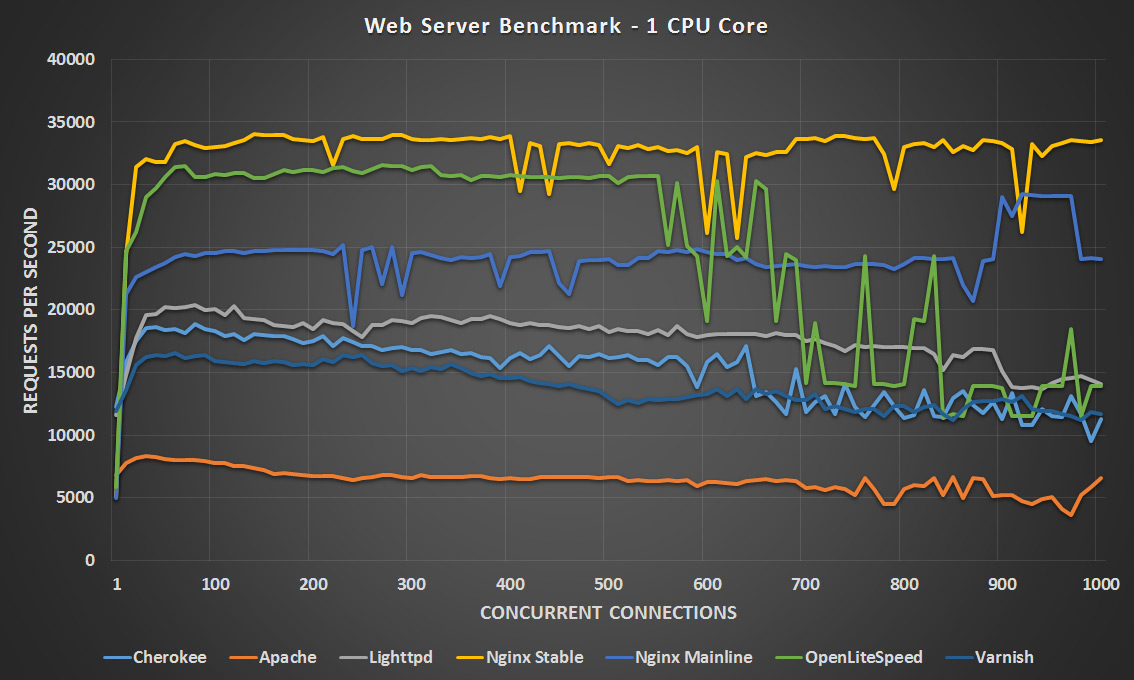
\includegraphics[scale=0.35]{web-server-performance-benchmark-1-cpu-core-1.jpg}
					\caption{Ilość obsługiwanych zapytań przy danej ilości otwartych połączeń. Źródło: Linux Web Server Performance Benchmark}
				\end{figure}
			\end{center}

			\begin{center}
				\begin{figure}[ht]
					\centering
					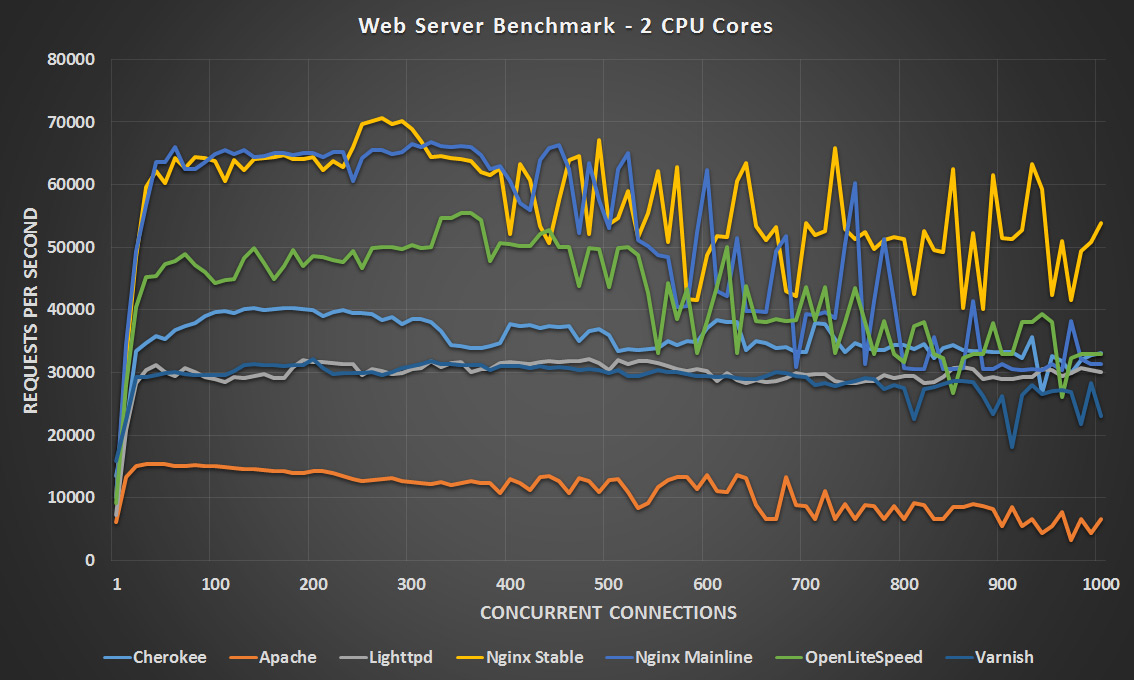
\includegraphics[scale=0.35]{web-server-performance-benchmark-2-cpu-cores-2.jpg}
					\caption{Ilość obsługiwanych zapytań przy danej ilości otwartych połączeń. Źródło: Linux Web Server Performance Benchmark}
				\end{figure}
			\end{center}
		
			\subsection{Serwer aplikacji}
			Drugim rodzajem systemu jaki można wykorzystać to serwer aplikacji działający na protokole HTTP. Najpopularniejsze\footnote{https://plumbr.eu/uncategorized/most-popular-java-ee-servers-2016-edition} aplikacje to: Tomcat\footnote{https://tomcat.apache.org/}, WildFly\footnote{http://wildfly.org/} (dawny JBoss) oraz Jetty\footnote{https://eclipse.org/jetty/}. Za ich pomocą można napisać aplikację np. w języku Java lub C++, która później służy do obsługi zapytań sieciowych. W ten sposób można stworzyć zaawansowane serwery sieciowe odpowiadające potrzebom implementowanego systemu.
		
			Porównanie wyżej wymienionych serwerów aplikacji można znaleźć w artykule Lightweight Java servers and developer view on the App Server\footnote{https://advantage.ibm.com/2015/09/22/lightweight-java-servers-and-developer-view-on-the-app-server-update/}.
		
			\begin{center}
				\begin{figure}[ht]
					\centering
					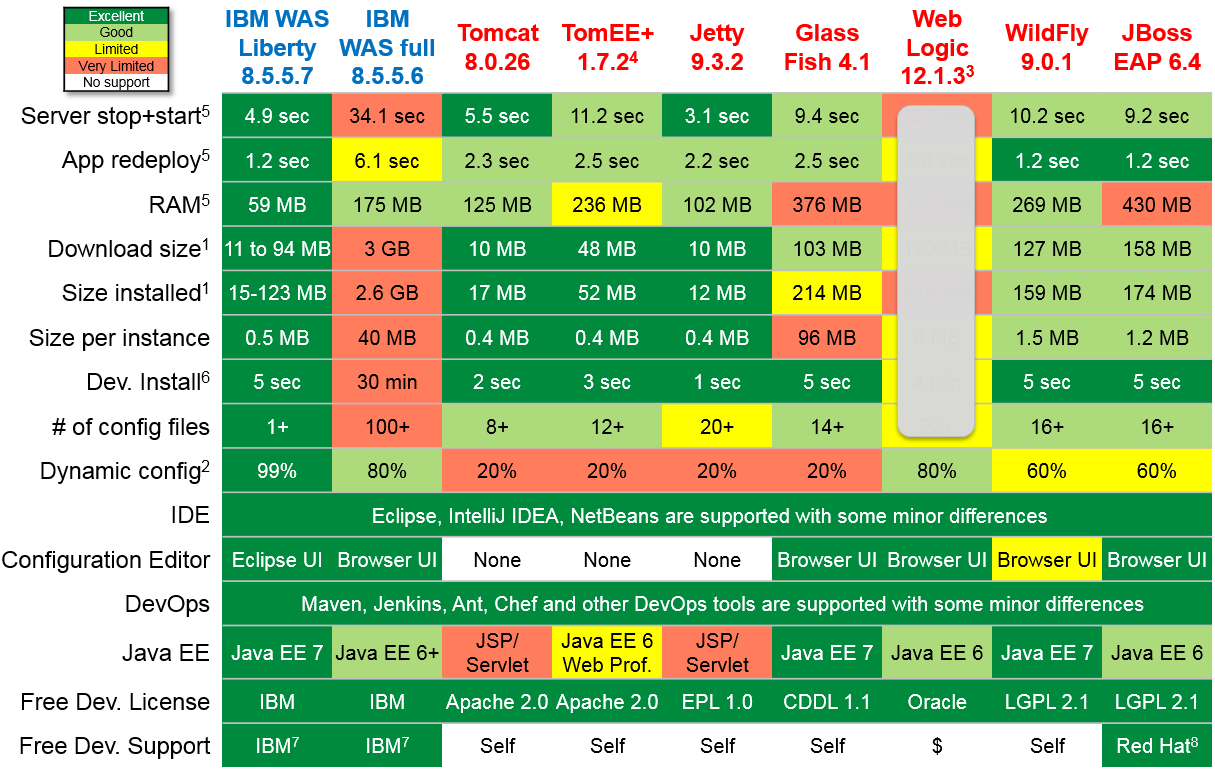
\includegraphics[scale=0.55]{weblogic-jboss-wildfly-websphere-liberty-tomee-tomcat-glassfish-comparison1.png}
					\caption{Porównanie popularnych serwerów aplikacji. Źródło: Lightweight Java servers and developer view on the App}
				\end{figure}
			\end{center}
	
	\chapter{Specyfikacja}
	
		\section{Początkowa specyfikacja}
		
			\subsection{Aplikacja mobilna}
			Podstawowe wymagania jakie aplikacja ma spełniać są następujące:
			\begin{itemize}
				\item zgodność z systemami Android w wersji 2.2 - 7.0
				\item komunikacja z serwerem przez HTTP
				\item szyfrowanie odpowiedzi z testu i przechowywanie ich w pamięci wewnętrznej telefonu
				\item bezpieczny sposób przechowywania odpowiedzi na telefonie
				\item ochrona oszukiwaniem poprzez nieuprawnione wyjście i powrót do wykonywanego testu
				\item logiczny i przyjazny dla użytkownika interfejs
			\end{itemize}
		
			\subsection{Aplikacja serwerowa}
			Wymagania aplikacji serwerowej są następujące:
			\begin{itemize}
				\item komunikacja przez HTTP
				\item duża wydajność przetwarzania zapytań sieciowych
				\item przetwarzanie i zapisywanie zapytań przychodzących z aplikacji mobilnych
				\item zachowanie możliwie wysokiej prostoty aplikacji serwerowej
			\end{itemize}
		
			\subsection{Dodatkowe programy}
			\begin{itemize}
				\item deszyfrator plików z odpowiedziami tworzonych przez aplikację mobilną
			\end{itemize}
		
		\section{Dodatki i zmiany}
		
			\subsection{Aplikacja mobilna}
			W trakcie implementacji i testowania systemu były wprowadzane zmiany w specyfikacji aplikacji mobilnej. Następujące zmiany to:
			\begin{itemize}
				\item komunikacja z serwerem poprzez HTTPS
				\item minimalna wersja obsługiwanego systemu Android zmieniona na 4.0
				\item lista z pytaniami zmieniona ze statycznej na dynamiczną
			\end{itemize}
			Dodatki to:
			\begin{itemize}
				\item odrzucanie połączeń przychodzących do użytkownika w trakcie testu
				\item długotrwałe przechowywanie parametrów konfiguracji takich jak imię, nazwisko, itd., w aplikacji
				\item wyświetlanie informacji dla użytkownika o procesach zachodzących w aplikacji
				\item nadanie aplikacji cyfrowego podpisu
				\item obfuskacja skompilowanego kodu źródłowego aplikacji
				\item testowanie osiągalności serwera HTTP
				\item weryfikacja aplikacji za pomocą SafetyNet
				\item automatyczna konfiguracja parametrów testu na podstawie danych otrzymanych z serwera
			\end{itemize}
		
			\subsection{Aplikacja serwerowa}
			Dodatki w specyfikacji aplikacji serwerowej wyglądają następująco:
			\begin{itemize}
				\item walidacja aplikacji mobilnych poprzez SafetyNet
				\item przesyłanie konfiguracji testu do aplikacji mobilnej
			\end{itemize}
		
			\subsection{Dodatkowe programy}
			\begin{itemize}
				\item konfigurator tworzący pliki konfiguracyjne dla aplikacji mobilnych
			\end{itemize}
	
	\chapter{Implementacja}
	
	Biorąc pod uwagę przeprowadzoną analizę problemu zdecydowano, że system do rozwiązywania testów musi być napisany od podstaw. Nie znaleziono przykładów otwartych systemów na tyle użytecznych, żeby można było użyć ich przy tworzeniu systemu. Systemy takie jak Quizowanie mają zamknięty kod i można się nimi sugerować jedynie w kwestii tworzenia interfejsu użytkownika.
	
		\section{Elementy aplikacji}
	
			\subsection{Widoki aplikacji}
		
			Wygląd aplikacji stanowi ważny element aplikacji. W początkowych fazach projektu rozmieszczenie elementów na ekranie telefonu komórkowego jak też ich estetyka wielokrotnie była zmieniana. Potrzebne było wypracowanie przejrzystego oraz przyjaznego dla studenta interfejsu aplikacji. W trakcie tworzenia aplikacji zauważono, że istotnym elementem jest zachowanie kompatybilności z różnymi wersjami systemu Android realizując jednolite i przewidywalne zachowanie się interfejsu.
			Na przykład nie można było zastosować kolorowania przycisków korzystając z metody setColorFilter obecnej we wszystkich wersjach systemu od Android 4.0 do Android 7.0. Efekt wywołania tej metody w systemach Android 4.0 do 4.4 był inny od efektu uzyskiwanego w systemach Android 5.0 i wyższych. Powodowało to brak kompatybilności pomiędzy tymi wersjami.\\
		
			Widoki jakie zostały zaimplementowane w aplikacji to:
			\begin{itemize}
				\item Widok główny\\
				Za jego pomocą użytkownik może wprowadzić swoje miejsce i rząd w jakim się znajduje, wektor wag służący do wyliczenia grupy na teście oraz kod testu. Na tym widoku można uruchomić również skaner kodów QR do automatycznego pobrania wektora wag i kodu testu oraz wyliczenia grupy na teście. Trzy dolne przyciski służą do wyjścia z aplikacji, ręcznego wyliczenia numeru grupy oraz przejścia do testu. Z tego widoku można również otworzyć menu, z którego można dostać się do widoku ustawień i widoku informacji.
			
				\item Widok ustawień\\
				Tutaj użytkownik może wprowadzić i zapisać w aplikacji swoje dane takie jak: imię, nazwisko, numer indeksu oraz nazwa przedmiotu. Opcjonalnie może wprowadzić inny adres serwera, na który aplikacja będzie przesyłać odpowiedzi użytkownika.
				
				\begin{figure}[ht]
					\centering
					\begin{subfigure}{.45\textwidth}
						\centering
						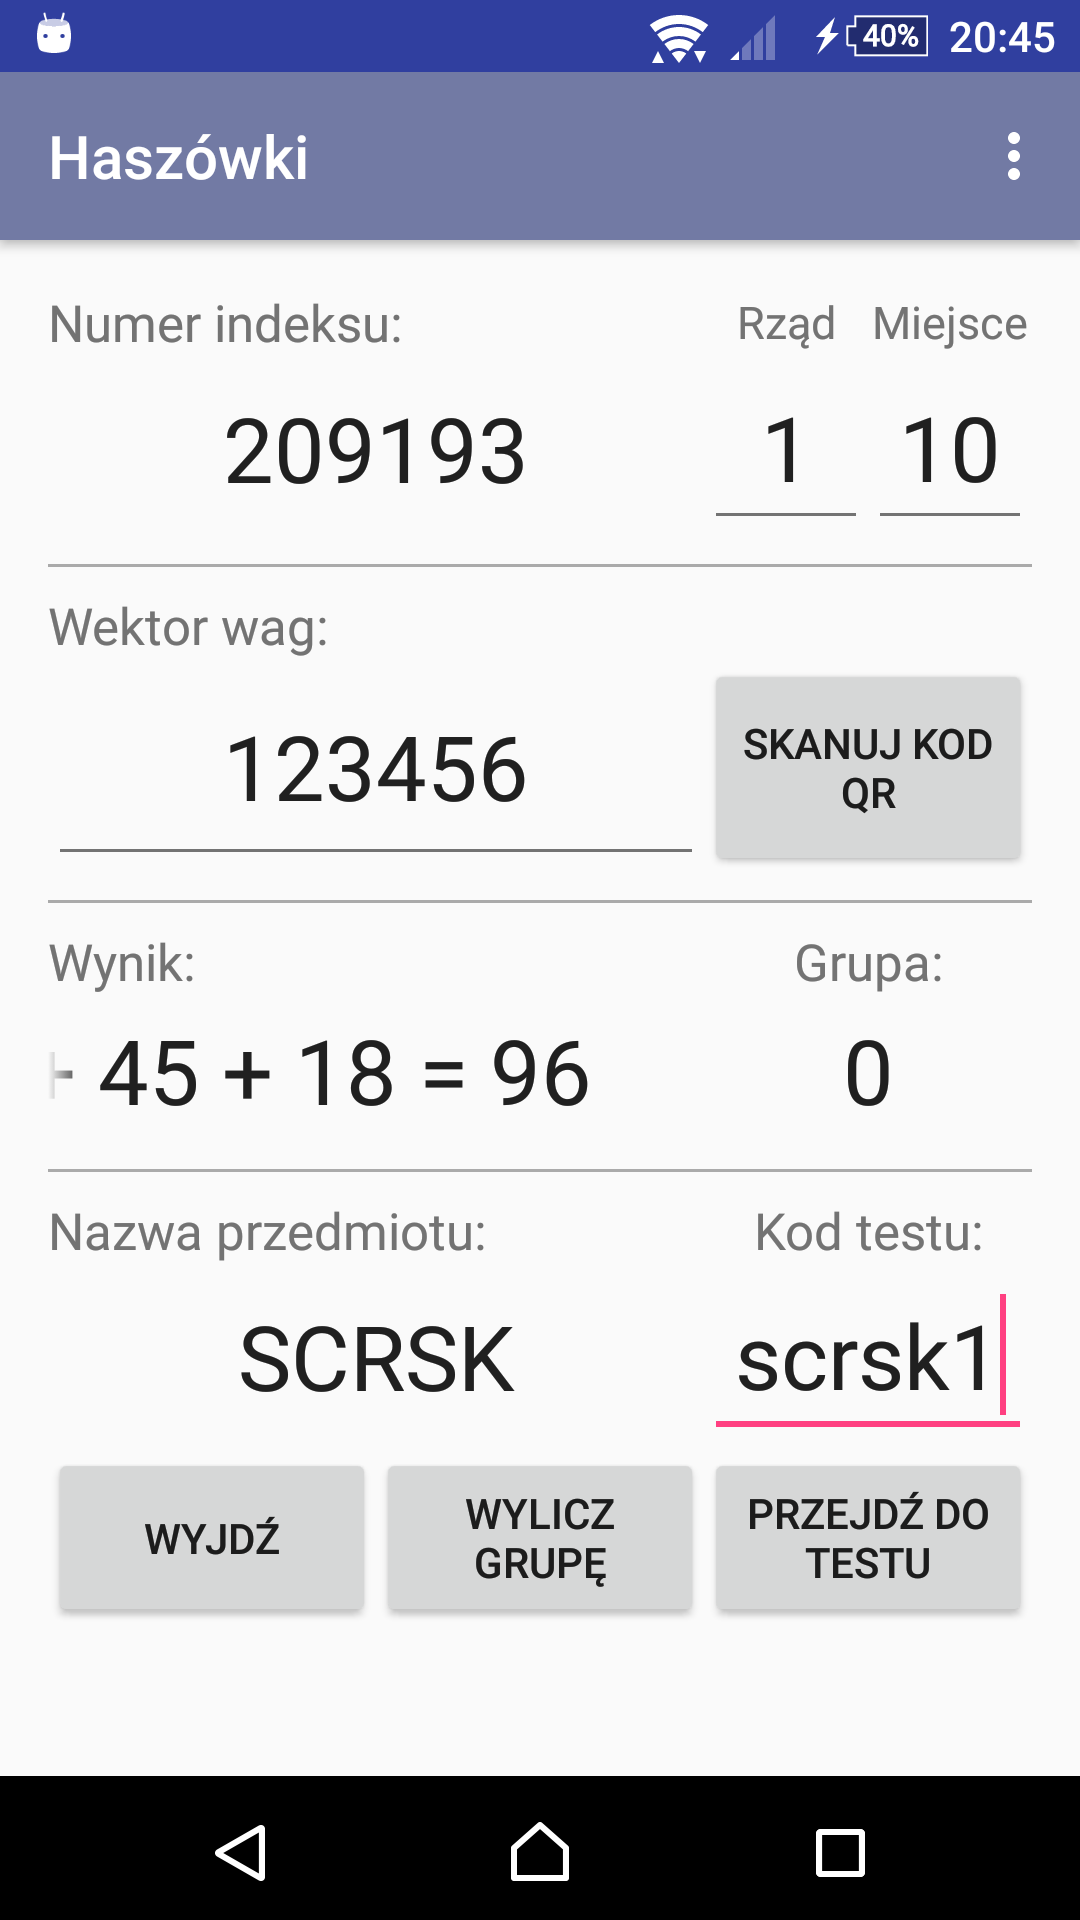
\includegraphics[width=.7\linewidth]{menu_glowne.png}
						\caption{Menu główne}
						\label{fig:menu_glowne}
					\end{subfigure}
					\begin{subfigure}{.45\textwidth}
						\centering
						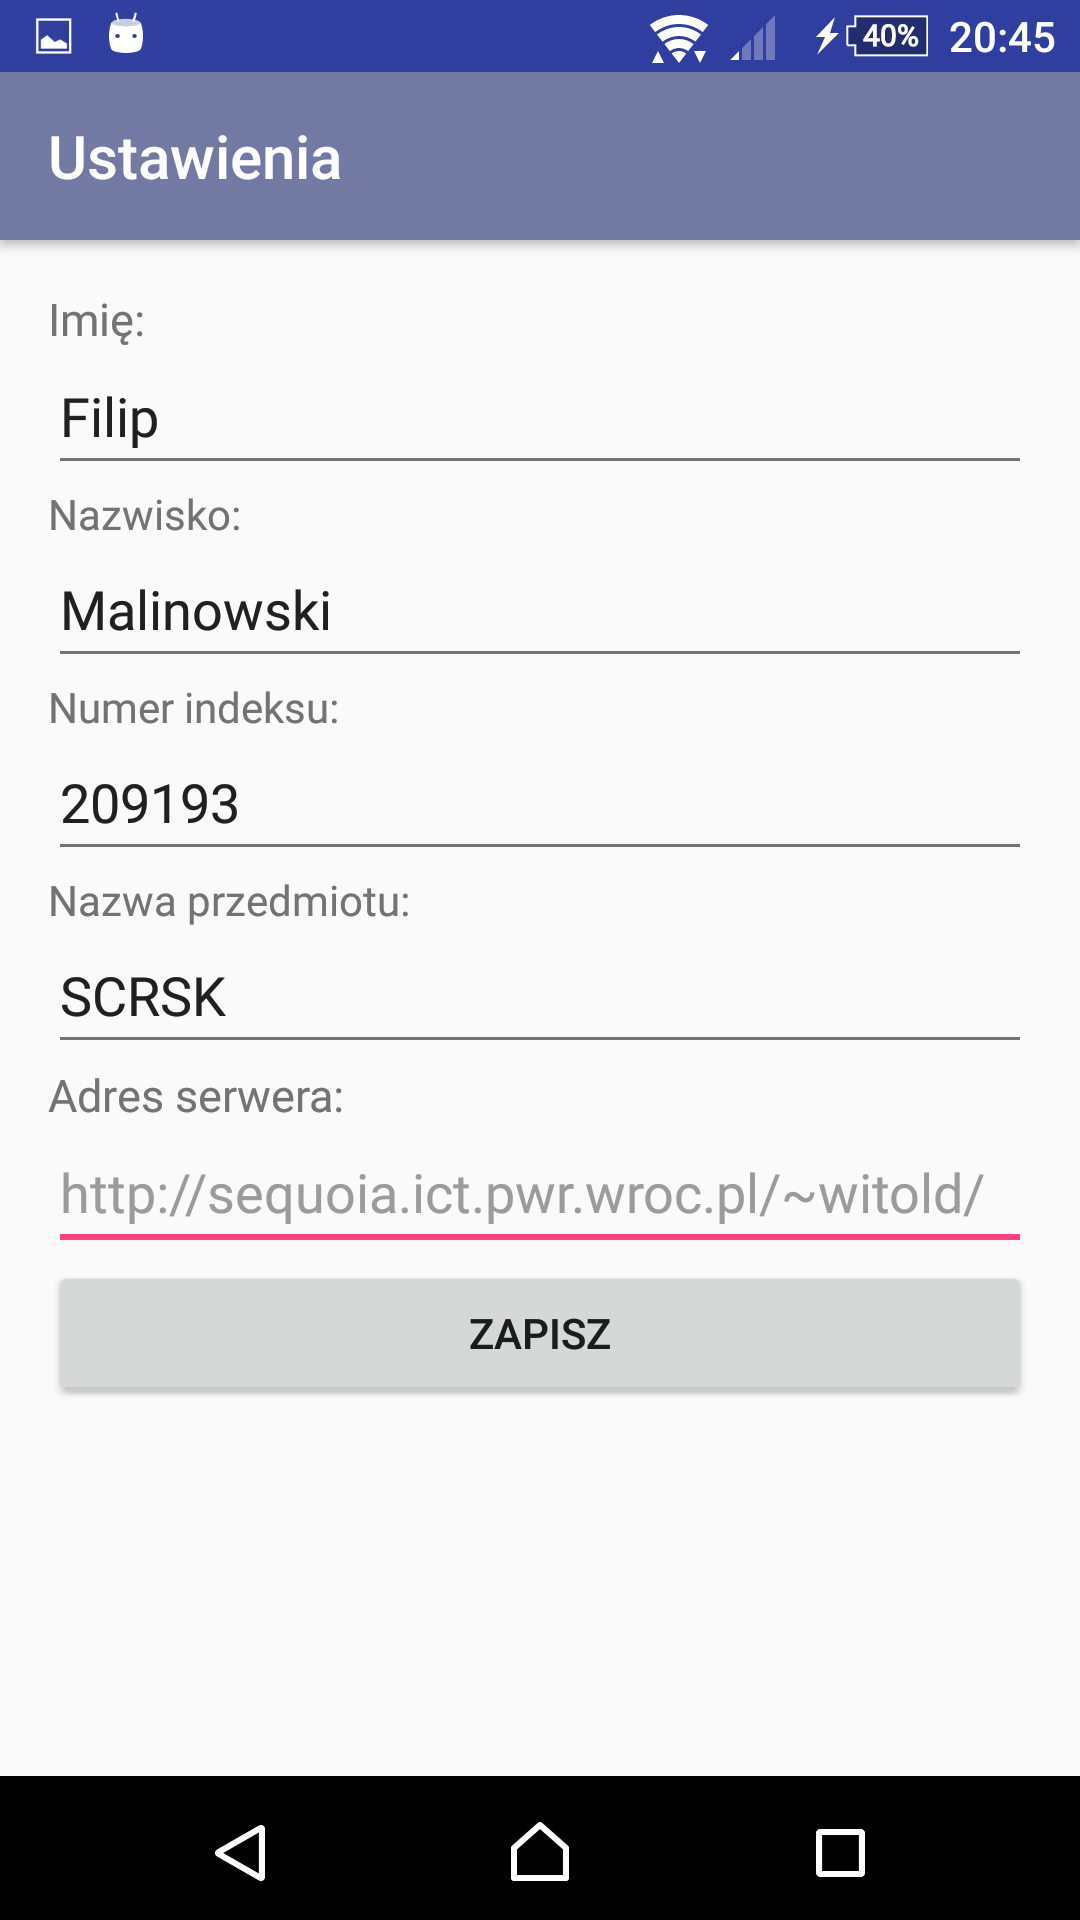
\includegraphics[width=.7\linewidth]{ustawienia.png}
						\caption{Ustawienia}
						\label{fig:ustawienia}
					\end{subfigure}
					\caption{Przykładowo skonfigurowane widoki menu głównego i ustawień}
					\label{fig:wyglad_aplikacji_1}
				\end{figure}
				
				\item Widok konfigurowania testu\\
				Tutaj użytkownik jest informowany o przebiegu konfiguracji testu. Aplikacja sprawdza osiągalność serwera, do którego wysyła odpowiedzi oraz pobiera plik konfiguracyjny zawierający takie dane jak: minimalna i maksymalna wersja aplikacji dopuszczona do testu oraz klucz do szyfrowania danych w plikach testu przechowywanych na telefonie użytkownika. Następnie porównuje dopuszczalną wersję aplikacji z aktualną wersją oraz zapisuje klucz szyfrowania.
				
				\item Widok testu\\
				W tym miejscu wyświetlany jest zestaw zakładek, po którym użytkownik może się poruszać i wchodzić w interakcje. UI użytkownika pozwala na przesuwanie ekranu w celu wyświetlenia innych pytań. Początkowo wyświetlana jest tylko jedna zakładka. Na zakładce pytania znajduje się: nr grupy użytkownika, nr pytania, przyciski: tak, nie, nie wiem do wysłania odpowiedzi, przyciski do dodawania pytań oraz do podsumowania testu. Na dole zakładki wyświetlany jest unikalny identyfikator sesji wygenerowany dla aktualnej sesji testowej otwartej na telefonie. Dodanie pytania wymusza przejście do następnego pytania. 
				
				\item Widok podsumowania\\
				Tutaj wyświetlana jest ilość poprawnie przesłanych odpowiedzi "tak", "nie" oraz "nie wiem" do serwera, oraz ilość odpowiedzi zapisanych w pliku testowym. W razie różnicy w odpowiedziach przesłanych do serwera, a zapisanych w pliku aplikacja wyświetla odpowiednie ostrzeżenie sugerujące użytkownikowi powrót do testu i ponowne przesłanie odpowiedzi. Na ekranie podsumowania wyświetlany jest przycisk pozwalający powrót do testu oraz przycisk kończący test powodujący powrót do menu głównego aplikacji.
				
				\item Widok informacji\\
				W tym widoku użytkownik może się dowiedzieć z jakiej wersji aplikacji korzysta.
				
				\begin{figure}[ht]
					\centering
					\begin{subfigure}{.45\textwidth}
						\centering
						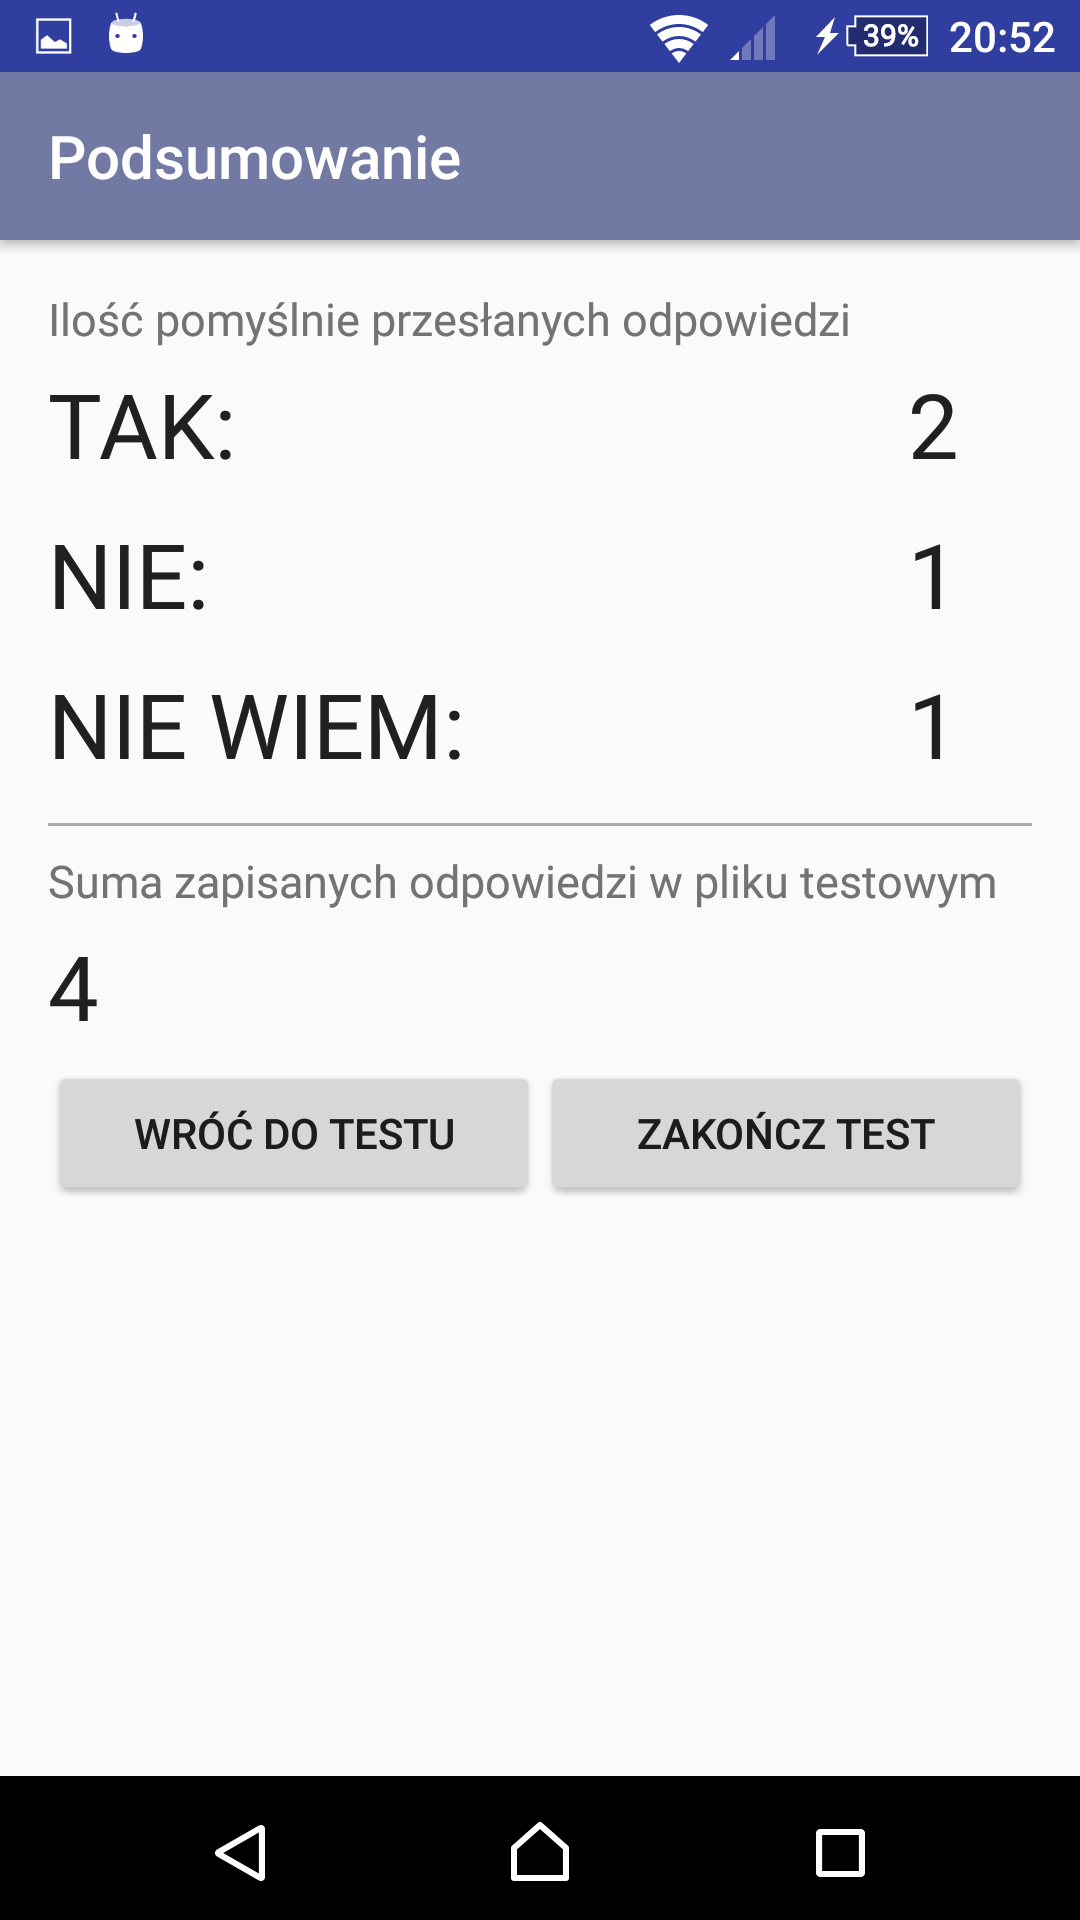
\includegraphics[width=.7\linewidth]{podsumowanie.png}
						\caption{Podsumowanie testu}
						\label{fig:podsumowanie}
					\end{subfigure}
					\begin{subfigure}{.45\textwidth}
						\centering
						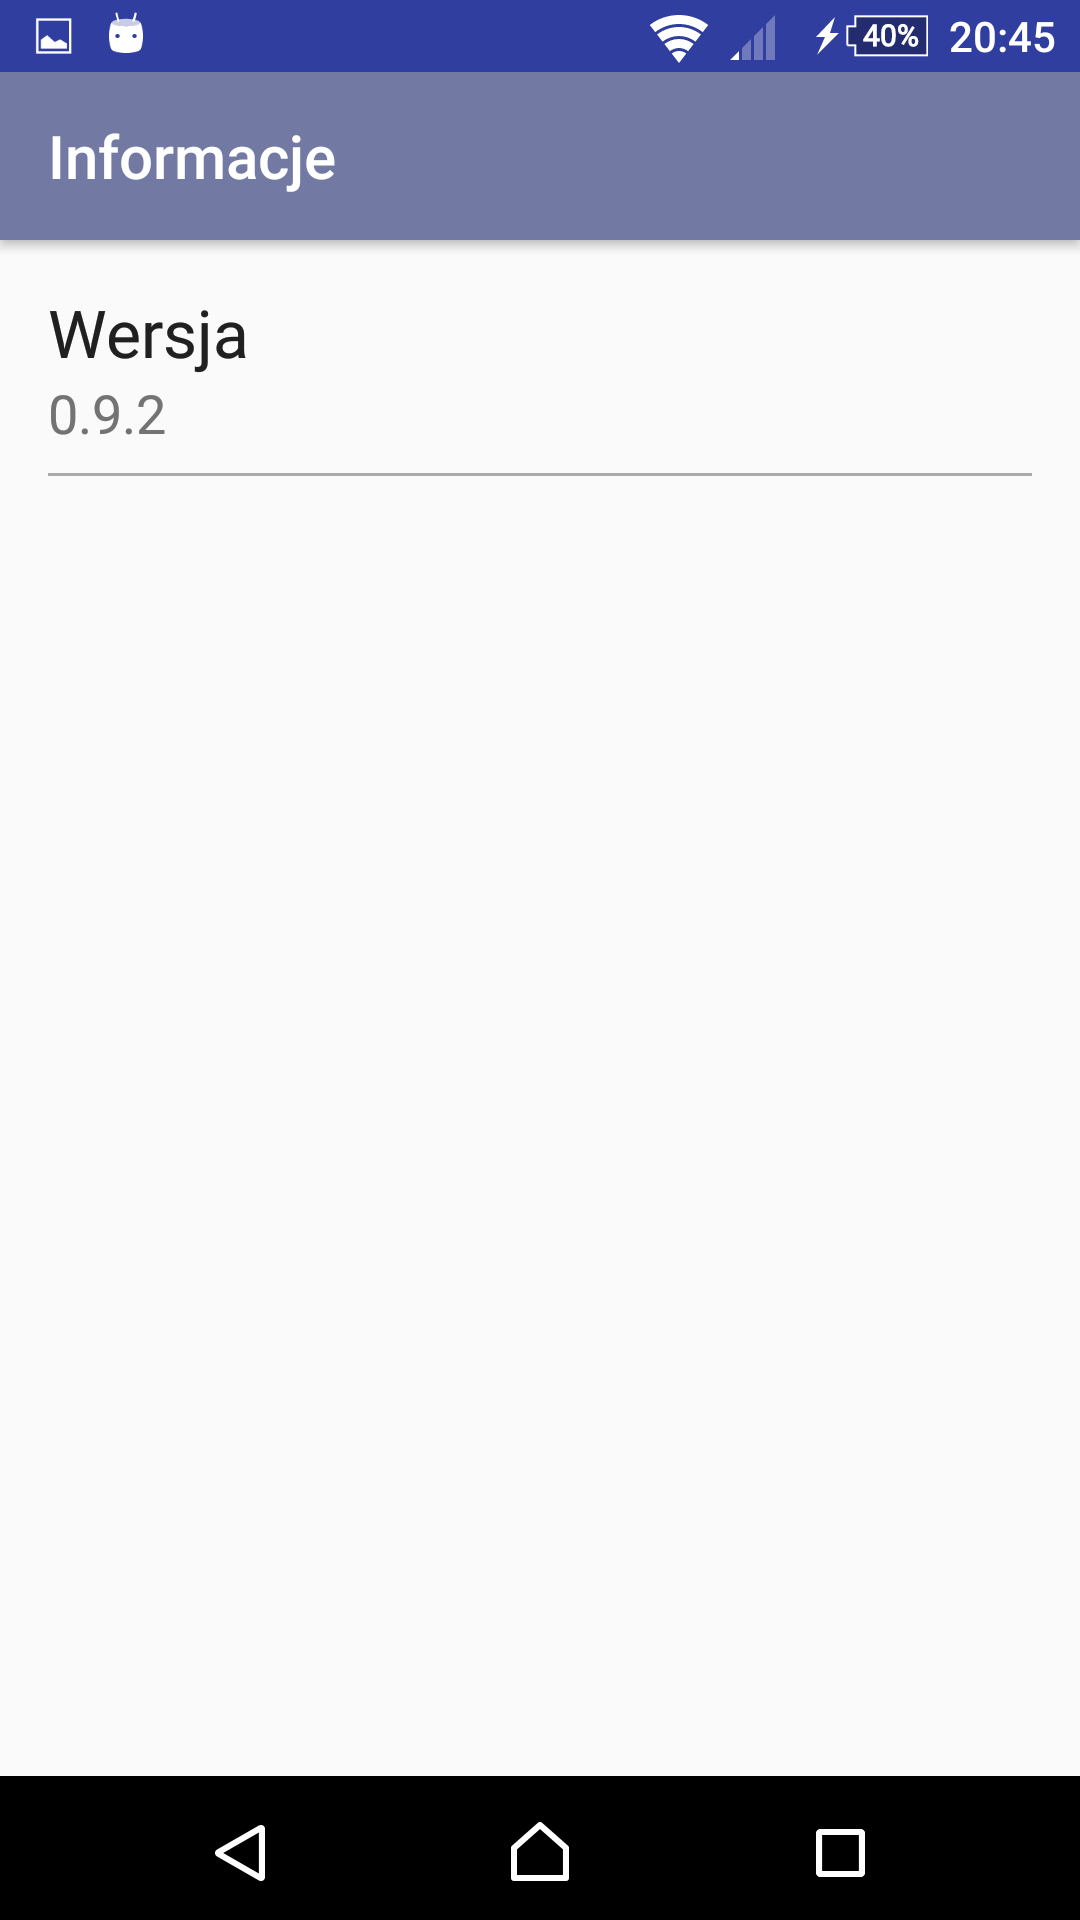
\includegraphics[width=.7\linewidth]{informacje.png}
						\caption{Informacje}
						\label{fig:informacje}
					\end{subfigure}
					\caption{Możliwe informacje wyświetlane na podsumowaniu i widoku informacji}
					\label{fig:wyglad_aplikacji_2}
				\end{figure}
				
			\end{itemize}
		
			\begin{center}
				\begin{figure}[ht]
					\centering
					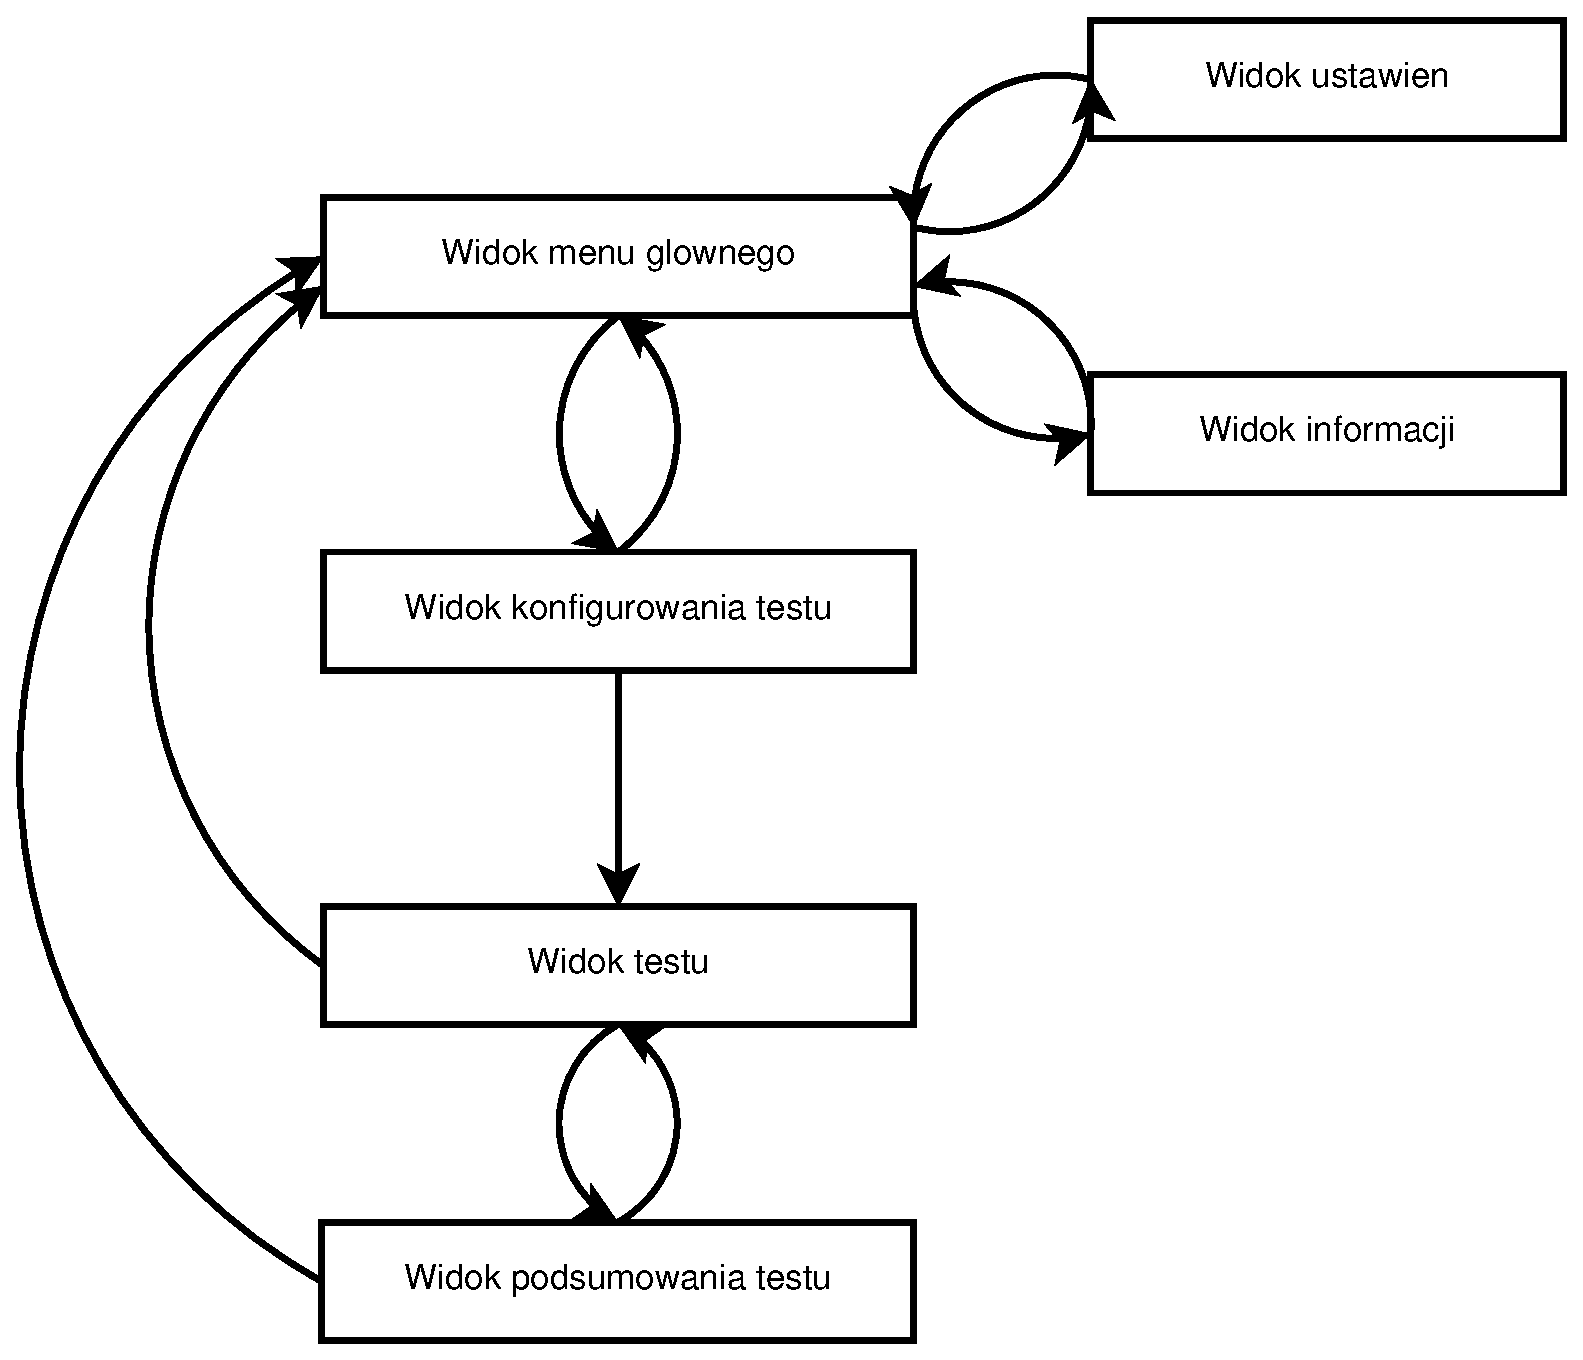
\includegraphics[scale=0.40]{diagram_zaleznosci_miedzy_widokami.eps}
					\caption{Zależności pomiędzy widokami informujące o tym jak użytkownik może się po nich poruszać}
				\end{figure}
			\end{center}
		
			\subsection{Interaktywne elementy na widokach}
		
				\paragraph{Rozwijane listy}
				zostały utworzone w widoku ustawień i widoku głównym. W widoku ustawień po kliknięciu na pole do edycji nazwy testu otwiera się okienko z przesuwalną listą, z której można wybrać nazwę kursu. W widoku głównym taka sama wizualnie lista wyświetla propozycje ID testu wygenerowane na podstawie nazwy kursu.
		
				\paragraph{Zmiennokształtne przyciski}
				służą do sygnalizowania asynchronicznych operacji zachodzących w trakcie konfiguracji i weryfikacji aplikacji. Za podstawę służy Android Circular Progress Button\footnote{https://github.com/flavioarfaria/circular-progress-button}, który został umieszczony na widoku ustawień. Przycisk ten w aplikacji zmienia swój kolor oraz wygląd sygnalizując:
				\begin{itemize}
					\item bezczynność - niebieski pusty przycisk
					\item przetwarzanie operacji - wirujące kółko
					\item powodzenie przetwarzania operacji - zielony przycisk z checkmark
					\item niepowodzenie przetwarzania operacji - czerwony przycisk 
				\end{itemize}
				Sygnalizowanie bezczynności zostało początkowo użyte dla jednej nieaktywnej funkcji, którą była walidacja aplikacji. Zielony kolor sygnalizuje powodzenie testowego połączenia z serwerem, poprawne pobranie pliku konfiguracyjnego oraz walidację klucza szyfrowania i dopuszczalny zakres wersji aplikacji.
				Czerwony kolor sygnalizuje niepowodzenie wyżej wymienionych operacji.
				Wirujące kółko trwa tak długo jak te asynchronicznie wykonywane operacje nie zakończą swojego działania.\\
				
				\begin{figure}[ht]
					\centering
					\begin{subfigure}{.3\textwidth}
						\centering
						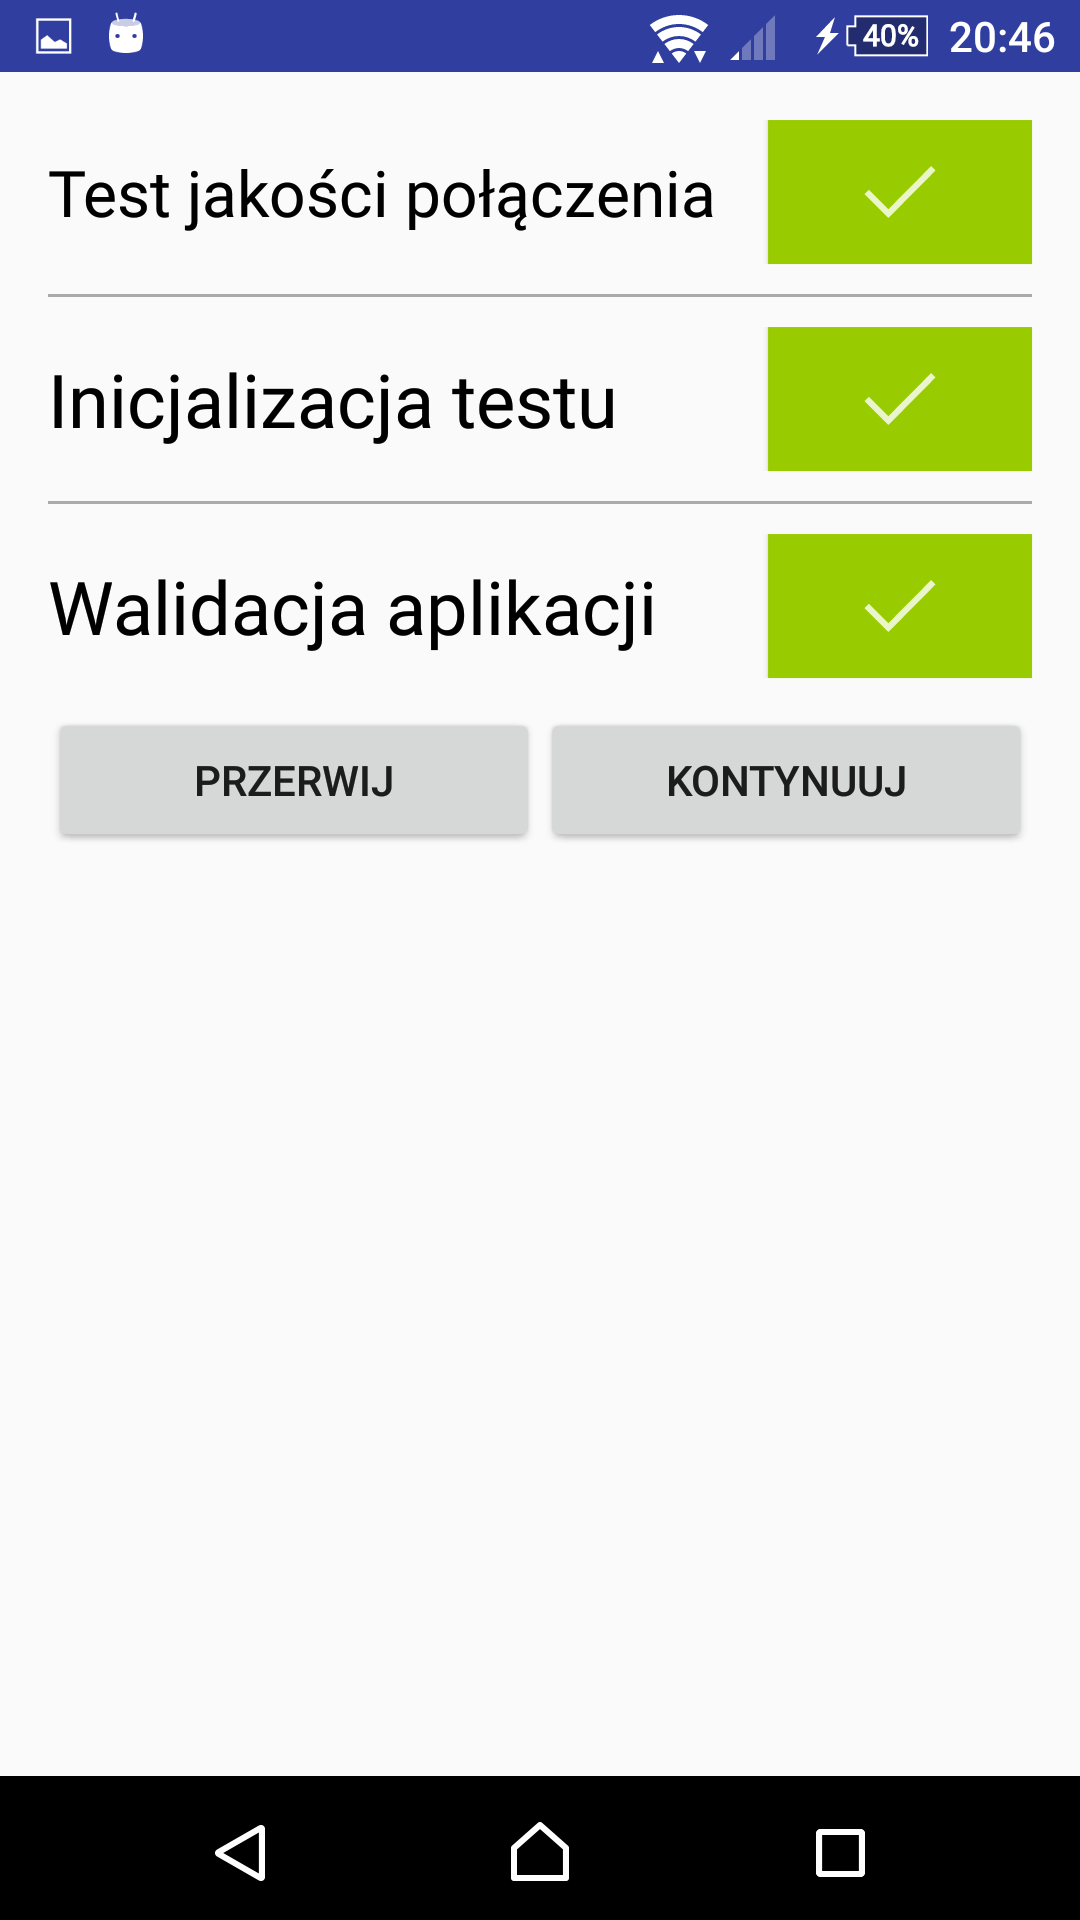
\includegraphics[width=.7\linewidth]{walidacja_wszystko_dobrze.png}
						\caption{Walidacja przeszła poprawnie}
						\label{fig:walidacja_poprawna}
					\end{subfigure}
					\begin{subfigure}{.3\textwidth}
						\centering
						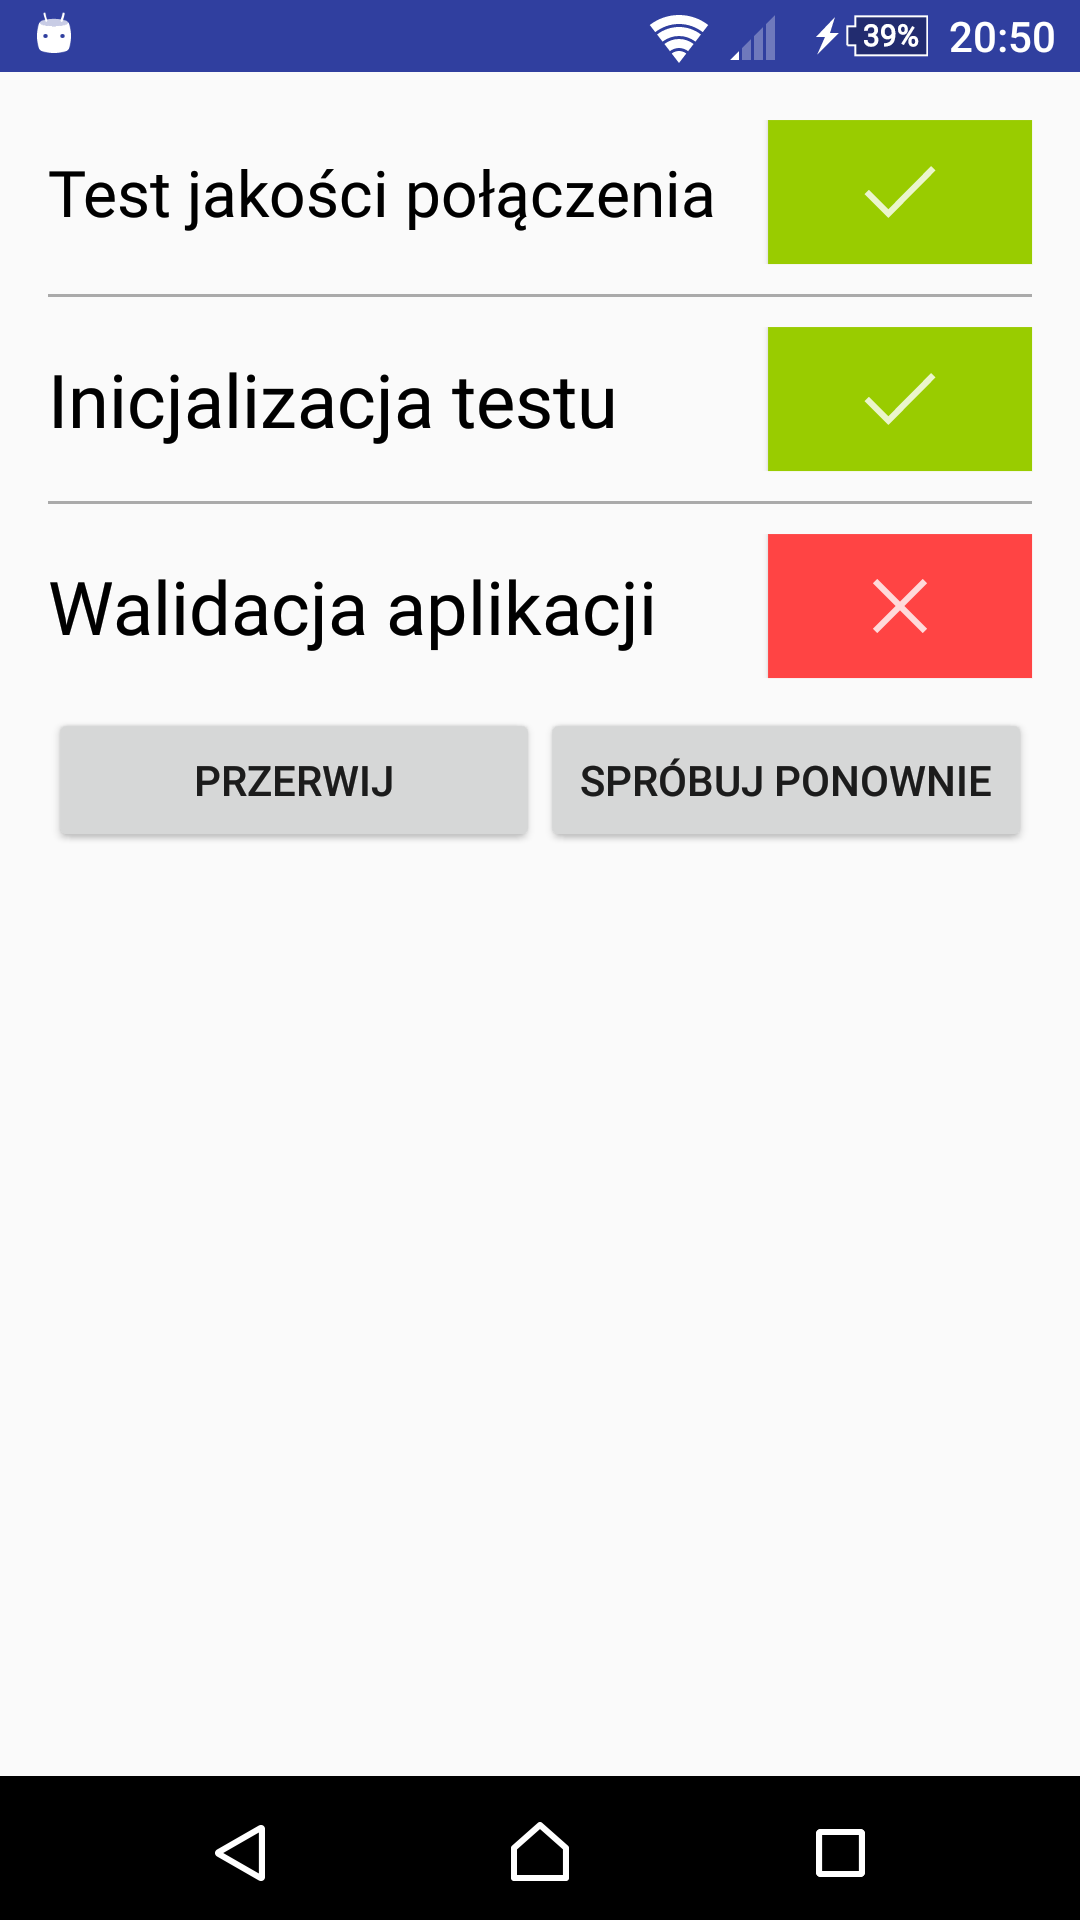
\includegraphics[width=.7\linewidth]{walidacja_niepoprawna_wersja_lub_klucz.png}
						\caption{Niepoprawna wersja lub klucz}
						\label{fig:walidacja_zly_klucz_wersja}
					\end{subfigure}
					\begin{subfigure}{.3\textwidth}
						\centering
						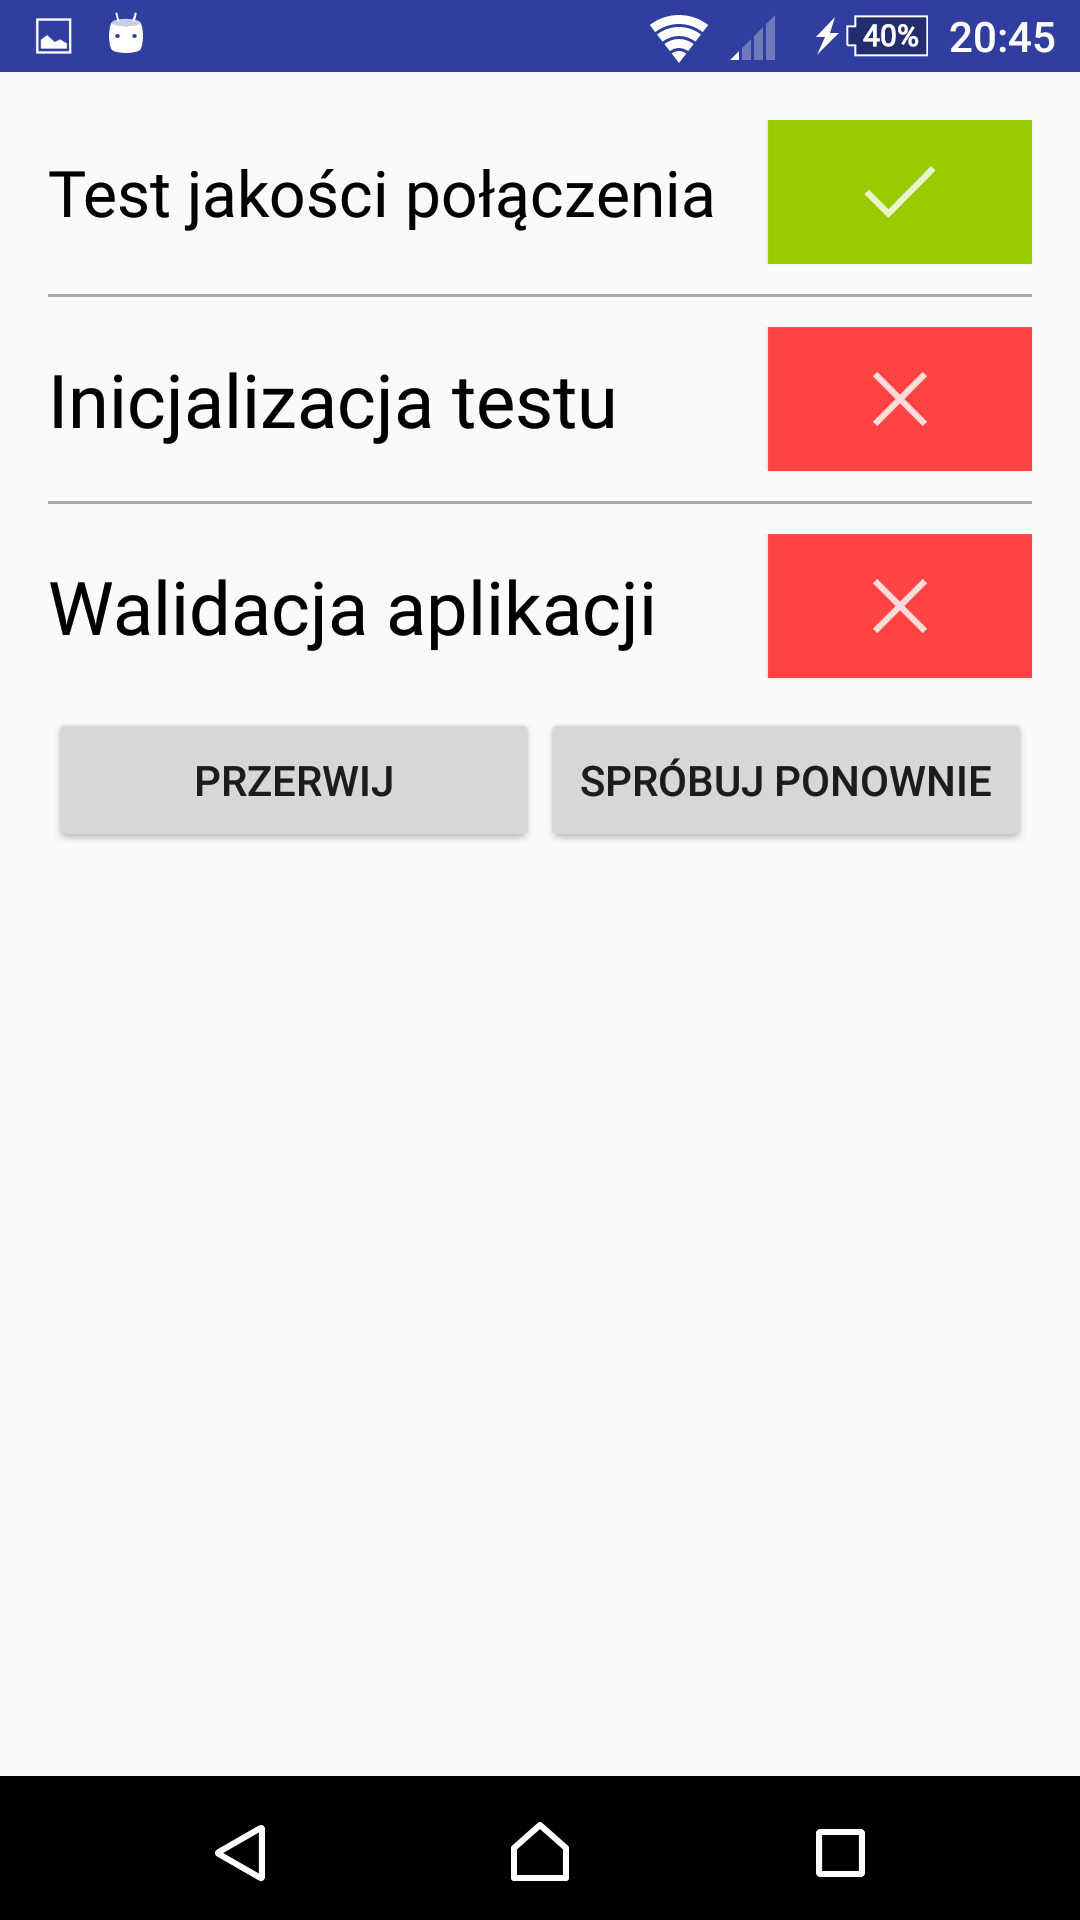
\includegraphics[width=.7\linewidth]{walidacja_brak_pliku_konfiguracyjnego.png}
						\caption{Brak pliku konfiguracyjnego na serwerze}
						\label{fig:walidacja_brak_pliku}
					\end{subfigure}
					\caption{Przykładowe wyniki etapu konfiguracji}
					\label{fig:wyglad_aplikacji_3}
				\end{figure}
				
				\paragraph{Przyciski zmieniające kolor}
				umieszczone są na kartach z odpowiedziami w aplikacji. Sygnalizują swoimi kolorami stan przetwarzania odpowiedzi użytkownika. Biały przycisk informuje o braku wybranej do tej pory odpowiedzi. Szary przycisk sygnalizuje poprawnie zapisaną odpowiedź do pliku testowego. Niebieski przycisk sygnalizuje poprawnie wysłaną odpowiedź na serwer.
				Jeżeli operacja zapisywania do pliku się nie powiedzie to przycisk pozostaje biały.
				Jeżeli operacja wysyłania do serwera się nie powiedzie to przycisk pozostaje szary. Użytkownik wtedy wie, że jego aktualna odpowiedź przechowywana jest jedynie lokalnie.\\
				
				\begin{figure}[ht]
					\centering
					\begin{subfigure}{.45\textwidth}
						\centering
						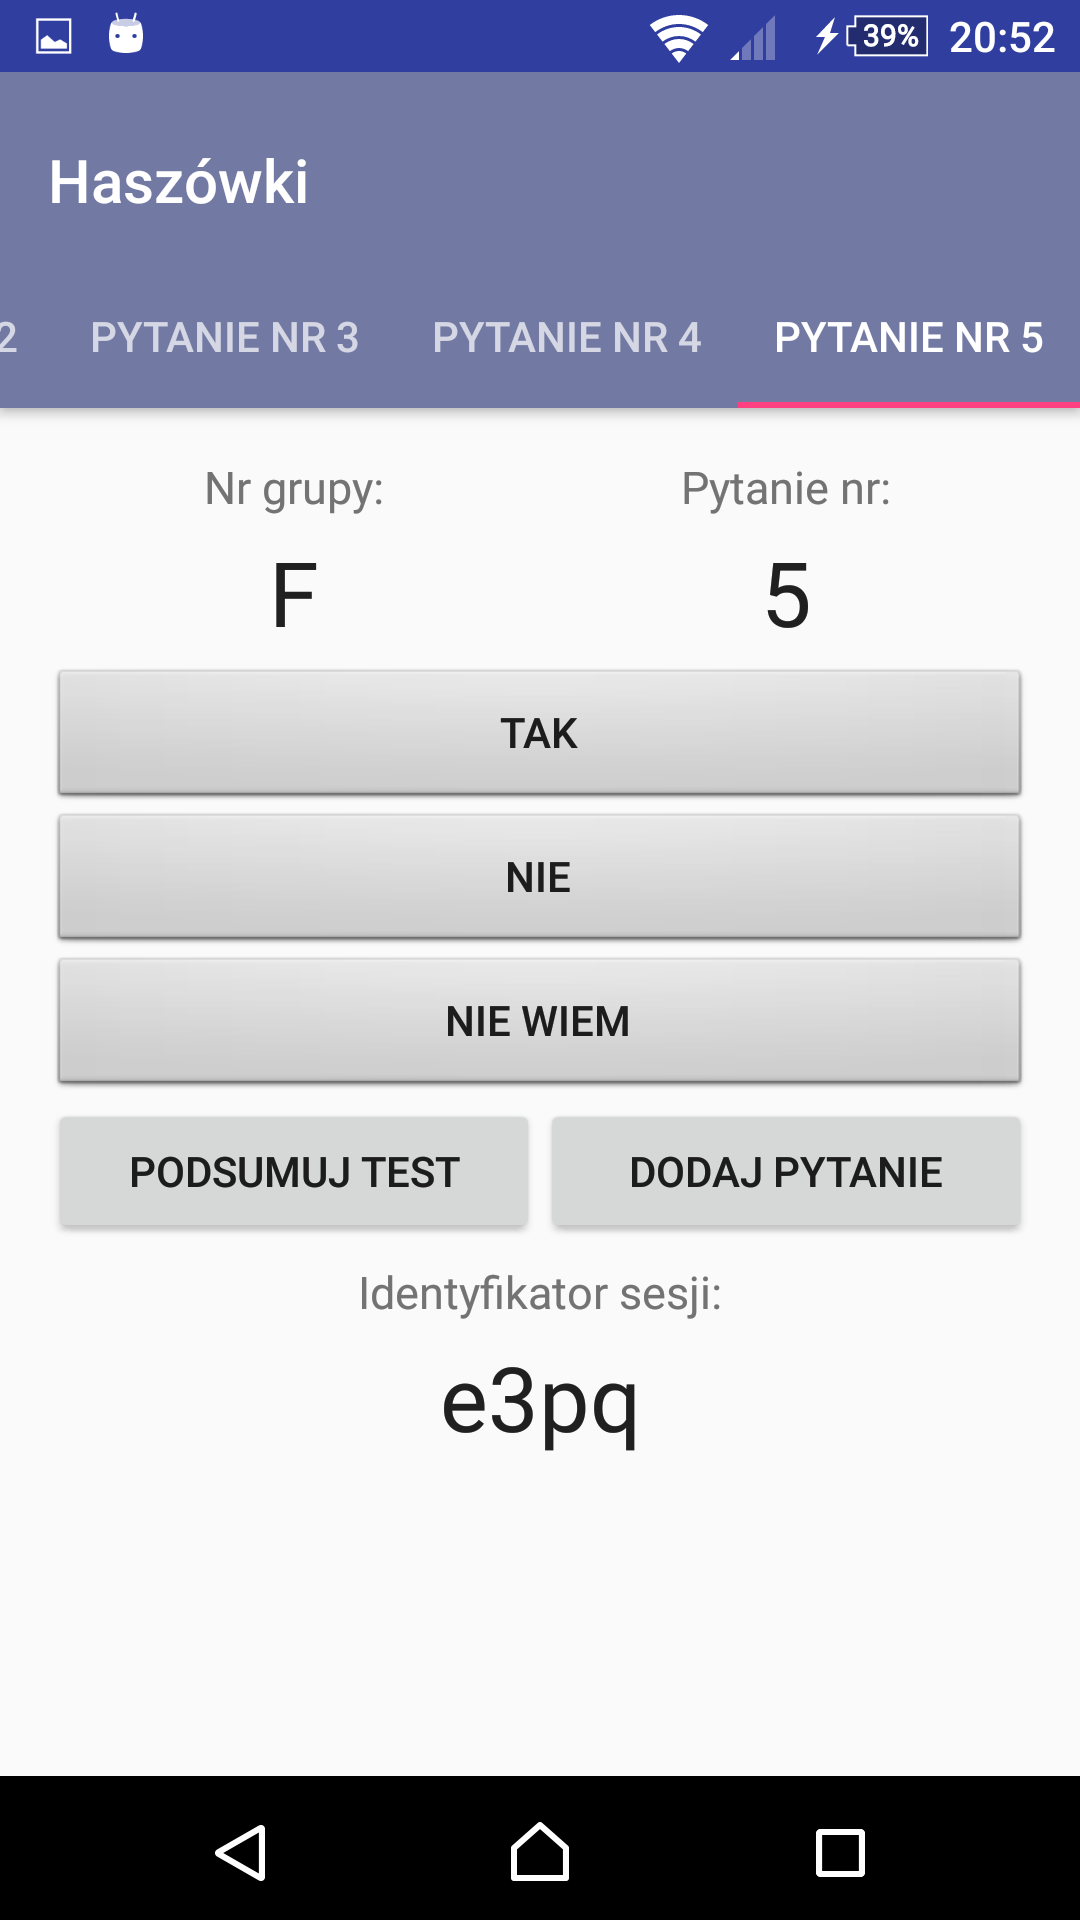
\includegraphics[width=.7\linewidth]{karta_pytania_odpowiedziana.png}
						\caption{Wybrana odpowiedź "tak"}
						\label{fig:odpowiedz_wybrana}
					\end{subfigure}
					\begin{subfigure}{.45\textwidth}
						\centering
						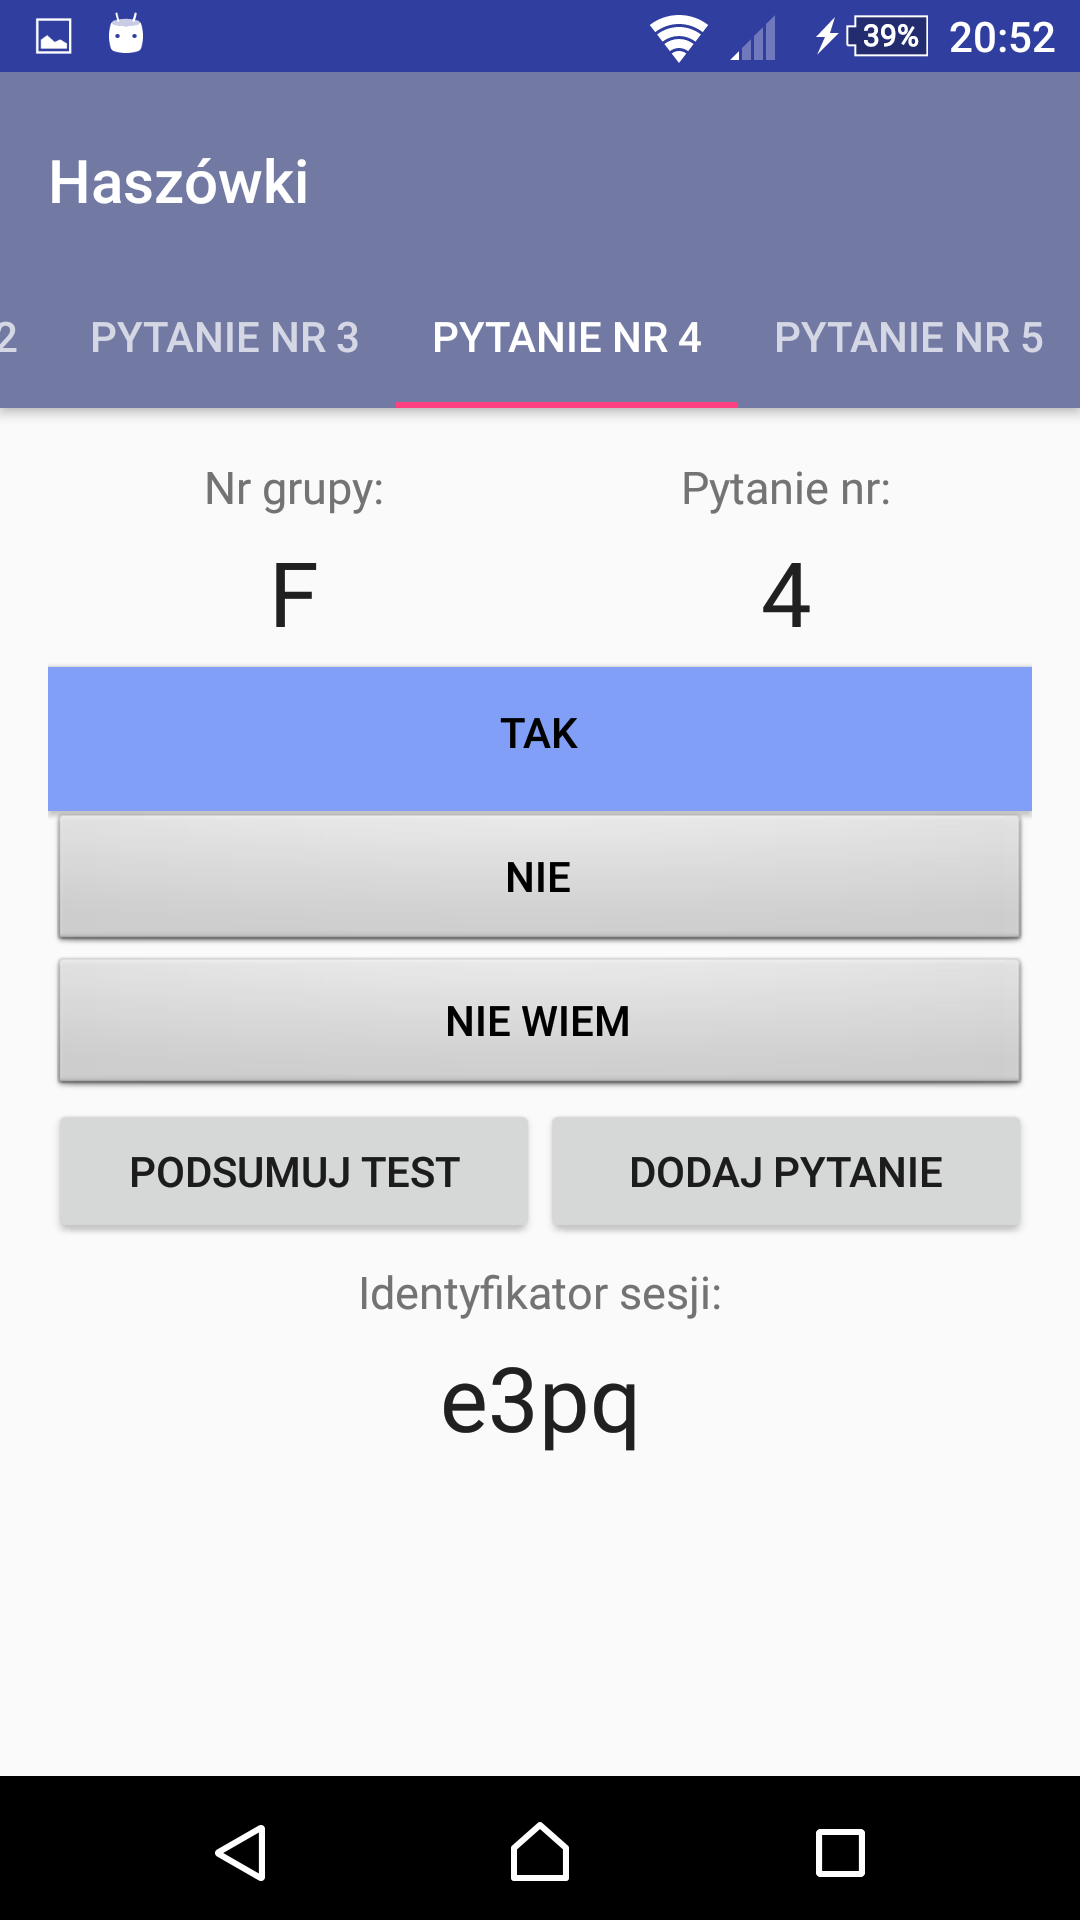
\includegraphics[width=.7\linewidth]{karta_pytania_nieodpowiedziana.png}
						\caption{Brak wybranej odpowiedzi}
						\label{fig:odpowiedz_niewybrana}
					\end{subfigure}
					\caption{Widok testu}
					\label{fig:wyglad_aplikacji_4}
				\end{figure}
				
				
			\begin{absolutelynopagebreak}
				\subsection{Powiadomienia}
		
				Istotnym elementem aplikacji okazały się być powiadomienia pozwalające na zrozumienie użytkownikowi zdarzeń występujących w aplikacji. Dzięki wypracowaniu zestawu chmurek oraz monitów użytkownik jest na przykład informowany o:
				\begin{itemize}
					\item wprowadzeniu nr indeksu o niepoprawnej długości,
					\item nie wprowadzeniu swojego imienia, nazwiska, kursu, indeksu,
					\item wprowadzeniu niepoprawnego wektora wag (równego 0),
					\item nie wprowadzeniu swojego miejsca i rzędu,
					\item braku dostępu do sieci,
					\item braku łączności z serwerem,
					\item niedotarciu do serwera danych odpowiedzi, itd.
				\end{itemize}
			\end{absolutelynopagebreak}
			
			\subsection{Komunikacja internetowa}
			
			Z tego powodu, że w niezabezpieczonej sieci WiFi Politechniki Wrocławskiej odblokowane są jedynie porty służące do obsługi poczty i protokołu HTTP to do komunikacji internetowej wykorzystano protokół HTTP. Odpowiedzi są wysyłane na zasadzie pobierania nagłówka pliku konfiguracyjnego XML z odpowiedziami umieszczonymi w query string. Kod otrzymany po wykonaniu zapytania jest następnie interpretowany, a jego wartość decyduje o powiadomieniu użytkownika o poprawnym lub niepoprawnym wysłaniu odpowiedzi do serwera.
		
			\subsection{Szyfrowanie plików}
		
			Początkowo pliki były szyfrowane algorytmem DES z kluczem przechowywanym w aplikacji. Było to jednak rozwiązanie niebezpieczne, ponieważ klucz szyfrowania można było uzyskać po zdekompilowaniu aplikacji. Pierwszym ulepszeniem zaimplementowanym w aplikacji było zastosowanie metody "security by obscurity", gdzie klucz szyfrowania zmieniał się w trakcie działania programu. W ten sposób sprawa jego uzyskania została utrudniona. Następnie w aplikacji zaimplementowano pobieranie dokumentu XML z ustawieniami testu. W tym dokumencie znajdował się klucz szyfrowania wykorzystywany później w algorytmie DES. W dalszym etapie wykorzystano szyfrowanie algorytmem RSA, którym zastąpiono algorytm DES, a klucz w dokumencie XML został zamieniony na 4096 bitowy klucz publiczny algorytmu RSA.
		
			\subsection{Skaner QR}
			
			W aplikacji wykorzystano również skaner kodów QR. Wykorzystano do tego bibliotekę zxing\footnote{https://github.com/zxing/zxing} (Zebra Crossing). Pozwala ona nie tylko na skanowanie kodów QR ale również kodów kreskowych, kodów Aztec i innych. Skaner skanuje kod QR wyświetlany na ekranie przez rzutnik, automatyczne zapisując w aplikacji kodu testu i wektor wag. Po operacji skanowania wymusza wyliczenie nowego numeru grupy. Ułatwia to pracę z aplikacją potencjalnemu użytkownikowi oraz pozwala na zmniejszenie prawdopodobieństwa popełnienia błędu przez użytkownika przy wyliczaniu grupy na teście.
			
			\subsection{Baza danych}
			
			Do długotrwałego przechowywania danych w aplikacji wykorzystano bazę danych MySQL. W tym celu stworzono klasę imitującą bazę danych MySQL oraz klasę imitującą interfejs dostępowy do tej klasy. Interfejs został następnie wykorzystany do zapisywania informacji zawartych w widoku ustawień. Baza danych dodatkowo służy jako narzędzie do wymiany danych między widokami aplikacji. Baza danych służy do przechowywania danych użytkownika takich jak: imię, nazwisko, numer indeksu oraz inne parametry właściwe dla aktualnej sesji testu. 
			
			\subsection{Odrzucanie połączeń w trakcie testu}
			
			W trakcie testowania aplikacji na grupie studentów pojawiła się potrzeba automatycznego odrzucania przychodzących połączeń telefonicznych. W tym celu stworzono klasę na bazie wbudowanej BroadcastReceiver, która to odrzuca wszystkie przychodzące połączenia jeśli użytkownik jest w trakcie pisania testu. Do odrzucania połączeń wykorzystano kod z portalu Stack Overflow\footnote{https://stackoverflow.com/questions/7347871/how-to-reject-a-call-programatically-in-android}.
			
		\section{Programy dodatkowe}
		
			\subsection{Generator konfiguracji}
			Do tworzenia plików konfiguracyjnych napisany został konfigurator w języku Java. Pozwala na uruchomienie się tylko w linii poleceń. W parametrach wywołania tego programu podaje się kod testu, minimalną wersję aplikacji oraz maksymalną wersję aplikacji dopuszczoną do testu. Program generuje dwa pliki. Pierwszy jest dokumentem XML zawierającym klucz publiczny RSA plus dodatkowe parametry testu przeznaczone dla aplikacji Android. Drugi plik zawiera klucz prywatny RSA służący do rozszyfrowywania odpowiedzi zaszyfrowanych wcześniej kluczem publicznym.
			
			\subsection{Deszyfrator}
			Deszyfrator również został napisany w języku Java i umożliwia uruchomienie się jedynie w linii poleceń. Początkowa wersja deszyfratora korzystała z algorytmu DES, najpierw ze stałym kluczem zapisanym w aplikacji, potem z kluczem odczytywanym z pliku. Deszyfrowanie odbywało się za pomocą klucza symetrycznego. Ostatecznie stosuje algorytm RSA, a klucz prywatny do rozszyfrowywania pobiera z pliku. Korzysta przy tym z szyfrowania asymetrycznego.
			
			\subsection{Parser logów}
			Do przetwarzania logów serwera Apache wykorzystano skrypt napisany w języku AWK. Skanuje on logi serwera Apache w poszukiwaniu zarejestrowanych zapytań przysłanych z aplikacji mobilnych i umożliwia zapisanie ich w formacie użytecznym dla zarządcy systemu. Skrypt został napisany przez Promotora dr Witolda Paluszyńskiego.
			

	\chapter{Testowanie systemu}
	
	System został pomyślnie wykorzystany na Wydziale Mechanicznym (W-10), kierunku Automatyce i Robotyce na kursie Systemy Czasu Rzeczywistego i Sieci Komputerowe (SCRSK). Średnio z aplikacji korzystało około 90 osób na każdym z siedmiu wykonanych testów. Ponadto aplikacja została wykorzystana na testach na Wydziale Elektroniki (W-4), kierunku Automatyce i Robotyce na kursie SCR Systemy Operacyjne.

		\subsection{W-10, AiR, SCRSK}
		
		\begin{absolutelynopagebreak}
			
			\paragraph{Wykorzystanie obu form dostarczania odpowiedzi z testu:}
			
			\centering
			\trimbox{0cm 0cm 0cm -1cm}{
				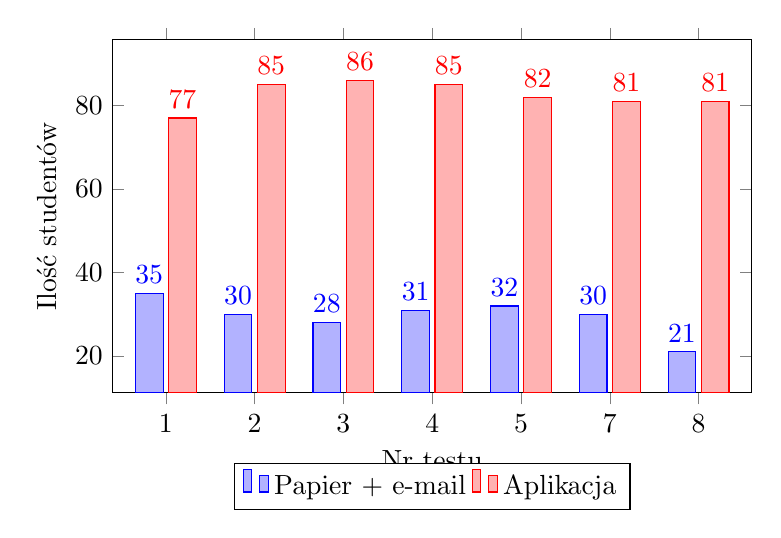
\begin{tikzpicture}
					\begin{axis}[
					ylabel=Ilość studentów,
					xlabel=Nr testu,
					symbolic x coords={1, 2, 3, 4, 5, 7, 8,},
					x tick label style={
						/pgf/number format/1000 sep=},
					enlargelimits=0.15,
					legend style={at={(0.5,-0.2)},
						anchor=north,legend columns=-1},
					ybar,
					enlarge x limits = 0.1,
					nodes near coords,
					width=0.8\textwidth,
					height=0.5\textwidth,
					]
					\addplot
					coordinates {(1,35) (2,30)
						(3,28) (4,31) (5,32)
						(7,30) (8,21)};
					\addplot
					coordinates {(1,77) (2,85)
						(3,86) (4,85) (5,82)
						(7,81) (8,81)};
					\legend{Papier + e-mail, Aplikacja}
					\end{axis}
				\end{tikzpicture}
			}
		
		\end{absolutelynopagebreak}
		
		\begin{absolutelynopagebreak}
			\paragraph{Ilość niepoprawnie wyliczonych grup przez studentów na testach:}
			
			\centering
			\trimbox{0cm 0cm 0cm -1cm}{
				\begin{tikzpicture}
				\begin{axis}[
				ylabel=Ilość błędnych grup,
				xlabel=Nr testu,
				symbolic x coords={1, 2, 3, 4, 5, 7, 8,},
				x tick label style={
					/pgf/number format/1000 sep=},
				enlargelimits=0.15,
				legend style={at={(0.5,-0.2)},
					anchor=north,legend columns=-1},
				ybar,
				enlarge x limits = 0.1,
				nodes near coords,
				width=0.8\textwidth,
				height=0.5\textwidth,
				]
				\addplot 
				coordinates {(1,2) (2,0)
					(3,2) (4,0) (5,1)
					(7,1) (8,1)};
				\end{axis}
				\end{tikzpicture}
			}
		
		\end{absolutelynopagebreak}
	
		\begin{absolutelynopagebreak}
			\paragraph{Ilość otrzymanych odpowiedzi na serwerze:}
			
			\centering
			\trimbox{0cm 0cm 0cm -1cm}{
				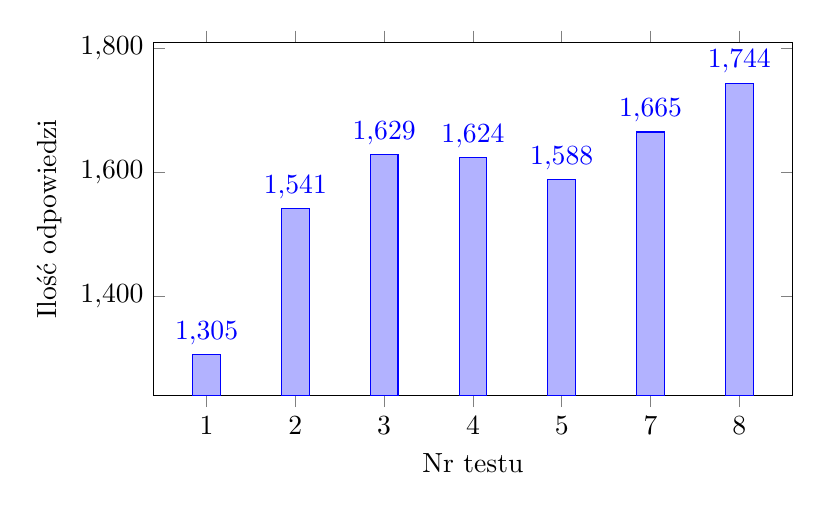
\begin{tikzpicture}
				\begin{axis}[
				ylabel=Ilość odpowiedzi,
				xlabel=Nr testu,
				symbolic x coords={1, 2, 3, 4, 5, 7, 8,},
				x tick label style={
					/pgf/number format/1000 sep=},
				enlargelimits=0.15,
				legend style={at={(0.5,-0.2)},
					anchor=north,legend columns=-1},
				ybar,
				enlarge x limits = 0.1,
				nodes near coords,
				width=0.8\textwidth,
				height=0.5\textwidth,
				]
				% papier
				\addplot 
				coordinates {(1,1305) (2,1541)
					(3,1629) (4,1624) (5,1588)
					(7,1665) (8,1744)};
				\end{axis}
				\end{tikzpicture}
			}
			
		\end{absolutelynopagebreak}
	
		\begin{absolutelynopagebreak}
			\paragraph{Ilość otrzymywanych odpowiedzi na sekundę:}
			
			\centering
			\trimbox{0cm 0cm 0cm -1cm}{
				\begin{tikzpicture}
				\begin{axis}[
				ylabel=Ilość otrzymywanych odpowiedzi na sekundę,
				xlabel=Nr testu,
				symbolic x coords={1, 2, 3, 4, 5, 7, 8,},
				x tick label style={
					/pgf/number format/1000 sep=},
				enlargelimits=0.15,
				legend style={at={(0.5,-0.2)},
					anchor=north,legend columns=-1},
				ybar,
				enlarge x limits = 0.1,
				nodes near coords,
				width=0.8\textwidth,
				height=0.5\textwidth,
				]
				% papier
				\addplot 
				coordinates {(1,10) (2,13)
					(3,11) (4,16) (5,12)
					(7,15) (8,11)};
				\end{axis}
				\end{tikzpicture}
			}
			
		\end{absolutelynopagebreak}
	
		\subsection{W-4, AiR, SCR Systemy Operacyjne}
		Statystyki pierwszego testu wyglądają następująco:
		\begin{itemize}
			\item wykorzystanie aplikacji: 78 osób
			\item wykorzystanie papieru + e-mail: 45 osób
			\item źle wyliczone grupy: 0
			\item ilość otrzymanych odpowiedzi: 5856
			\item ilość otrzymywanych odpowiedzi na sekundę: 29
		\end{itemize}
	
		\subsection{Błędy popełniane przy wyliczaniu grup}
		Statystyki błędów popełnianych przez studentów od 2012 roku:
		
		\centering
		\trimbox{0cm 0cm 0cm -1cm}{
			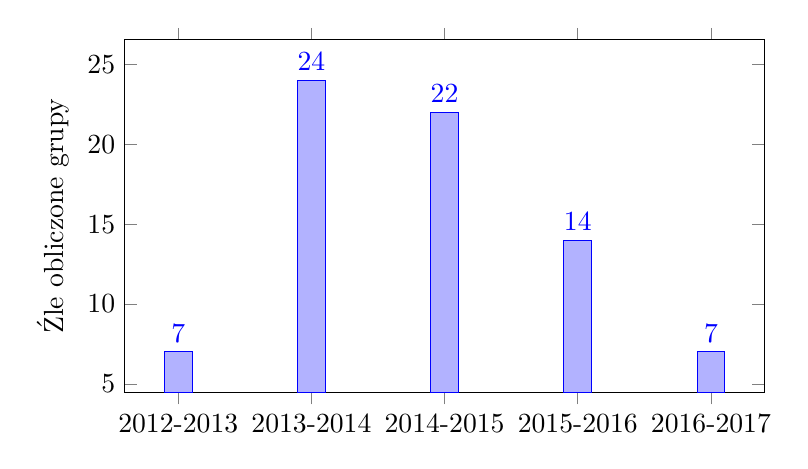
\begin{tikzpicture}
				\begin{axis}[
				ylabel=Źle obliczone grupy,
				symbolic x coords={2012-2013, 2013-2014, 2014-2015, 2015-2016, 2016-2017},
				x tick label style={
					/pgf/number format/1000 sep=},
				enlargelimits=0.15,
				legend style={at={(0.5,-0.2)},
					anchor=north,legend columns=-1},
				ybar,
				enlarge x limits = 0.1,
				nodes near coords,
				width=0.8\textwidth,
				height=0.5\textwidth,
				xtick=data,
				xticklabels={2012-2013, 2013-2014, 2014-2015, 2015-2016, 2016-2017},
				]
				\addplot 
				coordinates {(2012-2013,7) (2013-2014,24)
					(2014-2015,22) (2015-2016,14) (2016-2017,7)};
				\end{axis}
			\end{tikzpicture}
		}
	
		Aplikacja była testowana w okresie 2016-2017. Widać, że dzięki jej wykorzystaniu udało się zmniejszyć ilość popełnianych przez studentów błędów i wrócić do stanu z okresu 2012-2013.
	
			
\end{document}